\documentclass[fleqn,10pt]{wlscirep}
\usepackage[utf8]{inputenc}
\usepackage[T1]{fontenc}
\usepackage{booktabs}
\usepackage{multirow}
\usepackage{amsmath}
\usepackage{amssymb}
\usepackage{graphicx}
\usepackage{xcolor}
\usepackage{hyperref}
% xurl permits line breaks at any character inside \url{}. Without it the
% repository URL overflows the column and is silently clipped in the PDF,
% which is how the truncated URL in the original submission arose.
\usepackage{xurl}
\usepackage{array}
\usepackage{caption}
\usepackage{subcaption}
\usepackage{placeins}

% ── Float placement parameters ──────────────────────────────────────────────
\renewcommand{\topfraction}{0.85}
\renewcommand{\bottomfraction}{0.70}
\renewcommand{\textfraction}{0.10}
\renewcommand{\floatpagefraction}{0.75}
\setcounter{topnumber}{3}
\setcounter{bottomnumber}{2}
\setcounter{totalnumber}{6}

% ── Colour convention for the three neural architectures ────────────────────
\definecolor{agentblue}{HTML}{185FA5}
\definecolor{agentteal}{HTML}{1D9E75}
\definecolor{agentcoral}{HTML}{E8593C}

% ── Macros ──────────────────────────────────────────────────────────────────
\newcommand{\env}{\textsc{LakeGym~v5}}
\newcommand{\attentive}{\texttt{AttentivePPO}}
\newcommand{\mlpppo}{\texttt{MLP-PPO}}
\newcommand{\matchedmlp}{\texttt{MLP-matched}}
\newcommand{\ddqn}{\texttt{DDQN}}
\newcommand{\noop}{\texttt{NOOP}}
\newcommand{\cthirtytwo}{\texttt{COMPACT\_32KB}}
\newcommand{\csixtyfour}{\texttt{COMPACT\_64KB}}
\newcommand{\conehundredtwentyeight}{\texttt{COMPACT\_128KB}}
\newcommand{\phour}{\texttt{PARTITION\_HOUR}}
\newcommand{\pregion}{\texttt{PARTITION\_REGION}}
\newcommand{\ptype}{\texttt{PARTITION\_EVENT\_TYPE}}
\newcommand{\removep}{\texttt{REMOVE\_PARTITION}}

% ── Title and authors ───────────────────────────────────────────────────────
\title{Workload-Aware Data Lakehouse Maintenance Using Hierarchical Deep
Reinforcement Learning}

\author[1,*]{Omer Karim}
\author[1,*]{Omar Essameldin}
\author[1]{Omar Shrief}
\author[1,2]{Ahmed B. Zaky}

\affil[1]{Egypt-Japan University of Science and Technology (E-JUST),
Computer Science and Engineering Department, Alexandria, Egypt}
\affil[2]{Benha University, Faculty of Engineering at Shoubra,
Electrical Engineering Department, Cairo, Egypt}
\affil[*]{These authors contributed equally to this work}
\affil[$\dagger$]{\texttt{omer.karim@ejust.edu.eg},
\texttt{omar.isameldin@ejust.edu.eg},
\texttt{omar.shrief@ejust.edu.eg},
\texttt{ahmed.zaky@ejust.edu.eg}}
\affil[$\ddagger$]{Correspondence should be addressed to O.E.
(\texttt{omar.isameldin@ejust.edu.eg})}

% ── Abstract ────────────────────────────────────────────────────────────────
\begin{abstract}
Modern data lakehouses built on open table formats such as Apache Iceberg
accumulate small files and suboptimal partition layouts as data is
continuously ingested, degrading query performance over time.
Existing maintenance strategies rely on hand-crafted, workload-agnostic
rules that cannot adapt to shifting query distributions.
We present a hierarchical multi-agent framework that jointly optimises
compaction and partitioning decisions online: a rule-based
meta-controller evaluates per-step urgency scores and delegates to two
specialist reinforcement learning (RL) agents---a compaction agent and a
partition agent---each trained with a reward signal aligned to its
operational objective.
Within this framework we study three neural architectures: an
attention-based actor-critic (\attentive{}), a feedforward actor-critic
(\mlpppo{}), and a dueling double DQN (\ddqn{}), each trained under a
matched configuration with five independent random seeds.
Evaluation on \env{}, a simulation environment backed by a real Iceberg
table on Apache Spark, comprises 216 seeded runs with paired
non-parametric significance testing.
The best configuration (\ddqn{}) attains a mean global reward of 0.2105
(95\% CI [0.2050, 0.2155]), exceeding the strongest of 17 heuristic
baselines by $+$8.3\% (paired permutation $p = 0.001$, Cliff's
$\delta = +0.71$), with all five independent training runs individually
beating that heuristic.
The advantage persists on two held-out workloads exhibiting gradual
drift and concurrent query mixtures.
Ablation confirms a non-additive interaction between the two
specialists: removing compaction collapses partition pruning from 0.225
to 0.080 because data is never rewritten into the new layout.
Capacity-matched comparison shows the attention encoder confers no
significant advantage ($p = 0.54$), and direct inspection of its
attention weights reveals a static recency gate rather than
workload-transition sensitivity.
Across-seed variability differs sharply between architectures
(s.d.\ 0.0104 to 0.0403), demonstrating that single-checkpoint
evaluation is insufficient to rank architectures in this domain.
\end{abstract}

% ════════════════════════════════════════════════════════════════════════════
\begin{document}
\flushbottom
\maketitle
\thispagestyle{empty}

% ════════════════════════════════════════════════════════════════════════════
\section*{Introduction}
\label{sec:intro}
% ════════════════════════════════════════════════════════════════════════════

Data lakehouses combine the scalable storage of data lakes with the
transactional semantics of data warehouses through open table formats
such as Apache Iceberg\textsuperscript{1}, Delta
Lake\textsuperscript{2}, and Apache Hudi\textsuperscript{3}.
These formats store data as immutable Parquet files and maintain
metadata-level transaction logs, enabling ACID semantics on object
stores.
However, continuous ingestion generates large numbers of small files,
and the initial partition layout quickly becomes misaligned with the
actual query distribution as workloads evolve, increasing query scan
costs substantially.

State-of-practice maintenance is either manual or based on periodic
compaction schedules that are decoupled from query patterns.
Open-source auto-compaction heuristics\textsuperscript{1} trigger on
file-count thresholds but do not consider partition alignment.
Workload-aware approaches such as learned index
structures\textsuperscript{4} and automatic physical design
tools\textsuperscript{5} address layout optimisation offline and are
not designed for the continuous-ingestion regime of a lakehouse.
Reinforcement learning has been applied to query
optimisation\textsuperscript{6,7} and database
tuning\textsuperscript{8,9}, but not to joint compaction and
partitioning maintenance.

We argue that effective lakehouse maintenance requires \emph{joint},
\emph{online}, and \emph{workload-aware} decisions over both
compaction and partitioning.
This paper makes the following contributions.

\begin{itemize}
\item \textbf{Framework.} A hierarchical framework combining a
  rule-based arbitrator with two learned specialists, separating the
  when-to-act decision from the what-to-do decision. We are explicit
  that the arbitration tier is \emph{not} learned, and we quantify what
  that design choice costs.

\item \textbf{Environment.} \env{}, a simulation environment backed by
  a real Apache Iceberg table on Apache Spark with a structured,
  phase-shifting workload and a three-component reward function in which
  query latency is measured rather than modelled.

\item \textbf{Architecture study.} A comparison of three neural
  architectures (\attentive{}, \mlpppo{}, \ddqn{}) under a matched
  training configuration with five independent seeds each, evaluated
  with paired non-parametric tests, bootstrap confidence intervals, and
  effect sizes. We do not claim a universally best architecture; we
  report what each achieves and where they are statistically
  indistinguishable.

\item \textbf{Mechanism analyses.} Direct measurement of the attention
  encoder's behaviour, a capacity-matched control, an oracle
  meta-controller built on environment rollback, sensitivity analyses
  over every hand-chosen constant, and evaluation on two held-out
  workloads.

\item \textbf{Negative results.} Two findings that generalise beyond
  lakehouse maintenance: \emph{trajectory-identity leakage} when
  training offline RL on logs pooled from multiple behaviour policies,
  and a \emph{signal-below-noise} explanation for why greedy
  one-step meta-control fails where cooldown-based pacing succeeds.
\end{itemize}

\FloatBarrier

% ════════════════════════════════════════════════════════════════════════════
\section*{Related work}
\label{sec:related}
% ════════════════════════════════════════════════════════════════════════════

\textbf{Learned data layout.}
Qd-tree\textsuperscript{16} learns a block-partitioning scheme for
analytical workloads, and SageDB\textsuperscript{17} and learned index
structures\textsuperscript{4} synthesise data structures specialised to
an observed data and query distribution. These systems learn a
\emph{layout} offline for a distribution assumed to be known and
stationary, and reorganisation is a one-time or infrequent event. Our
setting differs in two ways: the distribution shifts during operation,
and every layout change is paid for continuously in rewrite cost. We
therefore learn a \emph{policy} over maintenance actions rather than a
layout, and the cost of acting is part of the objective.

\textbf{Reinforcement learning for database tuning.}
A substantial line of work applies RL to DBMS configuration:
OtterTune\textsuperscript{8} and CDBTune\textsuperscript{9} for knob
tuning, QTune\textsuperscript{20} for query-aware tuning,
LlamaTune\textsuperscript{21} for sample-efficient search,
HUNTER\textsuperscript{22} for hybrid online tuning,
HWTune\textsuperscript{23} for hardware-aware tuning,
CTuner\textsuperscript{24} for causal NoSQL tuning,
MLETune\textsuperscript{25} for LLM-guided knob tuning, and
multi-agent knob tuning for distributed
databases\textsuperscript{28}. In all of these the action adjusts a
configuration parameter; it does not rewrite data. Our actions are
physically destructive rewrites of Parquet files and evolutions of the
Iceberg partition specification, whose effects are delayed, partially
irreversible, and interact with each other. Self-driving
databases\textsuperscript{18} articulate the broader vision of
autonomous physical design that our work instantiates for the lakehouse
maintenance problem specifically.

\textbf{Learned query optimisation.}
Neo\textsuperscript{19}, SkinnerDB\textsuperscript{7} and
Re-Join\textsuperscript{6} learn to choose query plans. These operate
inside the execution of a single query, whereas maintenance decisions
change the physical state that all subsequent queries observe. The two
are complementary: a learned optimiser reduces the cost of a query given
a layout, while our agents change the layout the optimiser sees.

\textbf{Lakehouse storage and merge policy.}
Iceberg\textsuperscript{1}, Delta Lake\textsuperscript{2} and
Hudi\textsuperscript{3} define the transactional substrate;
LST-Bench\textsuperscript{14} provides workload-level benchmarking for
log-structured tables; and the Lakehouse
architecture\textsuperscript{15} frames the design space.
Dostoevsky\textsuperscript{12} analyses space--time trade-offs in
LSM-tree merging and is the closest prior treatment of compaction as an
optimisation problem, but it derives a static merge policy analytically
for a key-value store rather than learning an online policy for a
columnar table under a shifting query distribution.

\textbf{Hierarchical and multi-agent RL.}
FeUdal Networks\textsuperscript{27} learn a manager that sets subgoals
for a worker, and the multi-agent RL literature\textsuperscript{26}
surveys coordination mechanisms. Our meta-controller occupies the
manager role but is rule-based rather than learned. We treat this as a
deliberate simplification and evaluate it directly: we construct an
oracle arbitrator and a sensitivity sweep over its constants to bound
what the simplification costs.

\FloatBarrier

% ════════════════════════════════════════════════════════════════════════════
\section*{Results}
\label{sec:results}
% ════════════════════════════════════════════════════════════════════════════

\subsection*{Corrections to the training pipeline}
\label{sec:corrections}

While constructing the multi-seed evaluation protocol reported below, we
identified two defects in our offline training pipeline that materially
affected previously reported results. We describe them first because
they explain why the numbers in this paper differ from those in the
original preprint, and because both failure modes are, in our
assessment, easy to reproduce in other offline RL pipelines trained on
operational logs.

\textbf{Train/serve normalisation skew.}
Training standardised the \texttt{rows\_ingested} and
\texttt{ingestion\_rate} features by per-dataset $z$-scores, whereas the
deployed agent normalised them with fixed constants. Inference features
were therefore 10--50$\times$ outside the range seen during training,
saturating the network into an effectively constant
\conehundredtwentyeight{} policy. The apparent adaptivity of the
deployed agent was an out-of-distribution artefact rather than learned
behaviour.

\textbf{Trajectory-identity leakage.}
The staleness features $\delta_c$ (steps since last compaction) and
$\delta_p$ (steps since last partition change) encode \emph{which
behaviour policy generated a trajectory}: they remain near zero for
\texttt{AlwaysCompact} and grow without bound for
\texttt{No\_Maintenance}. When advantage-weighted regression is trained
on logs pooled across heuristics, these features provide a shortcut that
identifies the generating policy, and the network clones it instead of
reading table state. Holding table state fixed and varying only
$\delta_c$ from 0 to 30, the predicted probability of \noop{} rises from
0.00 to 0.94 --- a policy that is a function of trajectory provenance
rather than of the lakehouse.

Both defects are corrected by capping the staleness features, unifying
normalisation between training and serving, adding counterfactual
recovery trajectories, and sampling actions in a balanced manner during
offline training (Methods). Critically, \textbf{the environment itself
is unchanged}: re-evaluating the heuristic baselines under the corrected
pipeline reproduces the published values to within 0.003 (for example
\texttt{AlwaysCompact\_C128}: $0.1869 \rightarrow 0.1870$). The changes
in the RL results are therefore attributable to the pipeline
corrections and not to environment drift.

\FloatBarrier

\subsection*{Overall policy ranking}
\label{sec:ranking}

Table~\ref{tab:ranking} presents mean global reward with percentile
bootstrap 95\% confidence intervals for all policies on the 500-step
evaluation workload, together with the across-seed standard deviation.
Each RL architecture was trained with five independent random seeds and
each resulting agent evaluated on five episodes, giving 25 matched
episodes per policy. Environment seeds are a deterministic function of
(protocol, seed slot, episode) and are independent of the policy, so
every policy is evaluated on identical episodes and all comparisons are
paired.

\ddqn{} attains the highest mean global reward (0.2105, 95\% CI
[0.2050, 0.2155]), ahead of the best workload-aware heuristic
(\texttt{WorkloadAwareThreshold}, 0.1943) by $+$0.0162, a relative
improvement of $+$8.3\%. The 1{,}000-step protocol produces a
concordant ordering (Spearman $\rho = 0.964$, $p < 0.001$).

We emphasise two features of this table that were absent from our
original analysis. First, \textbf{not all RL configurations beat the
heuristics}: \mlpppo{} ranks below three heuristic policies. The
defensible claim is that the best RL configuration outperforms the best
heuristic, not that reinforcement learning as a class dominates.
Second, the across-seed standard deviation varies by a factor of four
between architectures (0.0104 for \ddqn{} versus 0.0403 for
\attentive{}), which is itself a result and is analysed below.

\begin{table}[!htbp]
\centering
\setlength{\tabcolsep}{4pt}
\begin{tabular}{clcccccc}
\toprule
\textbf{Rank} & \textbf{Policy} & \textbf{Reward} & \textbf{95\% CI} &
  \textbf{Seed s.d.} & \textbf{Latency (ms)} & \textbf{Files} &
  \textbf{Pruning} \\
\midrule
1 & \textbf{\ddqn{}} (RL)        & \textbf{0.2105} & [0.2050, 0.2155] & 0.0104 & 219.6 & 37.4 & 0.204 \\
2 & \texttt{WorkloadAwareThreshold} & 0.1943 & [0.1923, 0.1964] & 0.0020 & 323.6 & 49.9 & \textbf{0.248} \\
3 & \texttt{AlwaysCompact\_C128}    & 0.1903 & [0.1901, 0.1904] & 0.0002 & 197.9 & \textbf{22.1} & 0.000 \\
4 & \textbf{\attentive{}} (RL)   & 0.1823 & [0.1669, 0.1963] & 0.0403 & 331.1 & 51.6 & 0.225 \\
5 & \texttt{Threshold10\_C128}      & 0.1710 & [0.1708, 0.1712] & 0.0003 & 203.3 & 26.1 & 0.000 \\
6 & \textbf{\mlpppo{}} (RL)      & 0.1675 & [0.1579, 0.1772] & 0.0254 & 316.9 & 61.6 & 0.221 \\
7 & \texttt{Threshold10\_C64}       & 0.1273 & [0.1267, 0.1280] & 0.0011 & 321.3 & 46.8 & 0.000 \\
8 & \texttt{CompactOnly} (ablation) & 0.1202 & [0.1086, 0.1315] & 0.0428 & 314.0 & 48.4 & 0.000 \\
9 & \texttt{PartitionOnly} (ablation) & $-$0.1099 & [$-$0.1195, $-$0.1011] & 0.0116 & 3{,}643 & 793.0 & 0.080 \\
\bottomrule
\end{tabular}
\caption{\label{tab:ranking}\textbf{Policy ranking with uncertainty.}
  Mean global reward with percentile bootstrap 95\% confidence intervals
  (10{,}000 resamples) on the 500-step evaluation workload, 25 matched
  episodes per policy (5 training seeds $\times$ 5 episodes). ``Seed
  s.d.''\ is the standard deviation of the five per-seed means and
  quantifies training-run variability, which the confidence interval on
  the pooled mean does not. Hierarchical RL agents are shown in bold.
  Latency, file count and pruning ratio are episode-level means.}
\end{table}

\begin{figure}[!htbp]
\centering
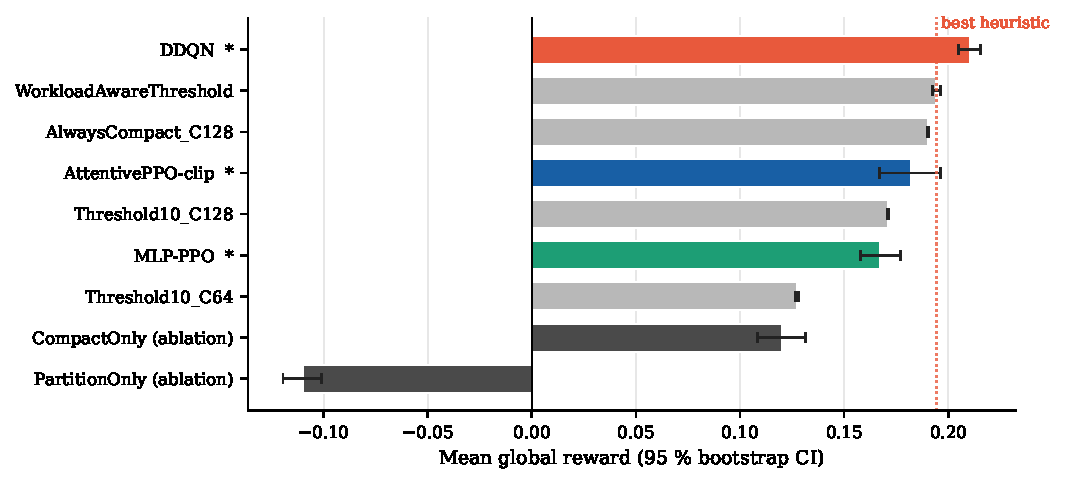
\includegraphics[width=0.86\linewidth]{charts/fig_ranking}
\caption{\label{fig:ranking}\textbf{Policy ranking with bootstrap 95\% confidence
  intervals.}
  Bars show mean global reward on the 500-step evaluation workload;
  whiskers are percentile bootstrap 95\% confidence intervals over 25
  matched episodes. Hierarchical RL agents are coloured by architecture
  (coral = \ddqn{}, blue = \attentive{}, teal = \mlpppo{}) and marked
  with an asterisk; heuristics are light grey and ablations dark grey.
  The dotted line marks the best heuristic. \ddqn{} is the only policy
  whose interval lies entirely above it; \mlpppo{} falls below three
  heuristics.}
\end{figure}

Table~\ref{tab:significance} reports paired significance tests for
\ddqn{} against every other policy. We use both the Wilcoxon
signed-rank test and an exact paired permutation test, report Cliff's
$\delta$ as a non-parametric effect size, and apply Holm--Bonferroni
correction within the comparison family. \ddqn{} significantly
outperforms every other policy evaluated
($p_{\text{Holm}} \leq 0.0018$), and all five of its independently
trained seeds individually exceed the best heuristic (per-seed range
0.198--0.224).

\begin{table}[!htbp]
\centering
\begin{tabular}{lccccl}
\toprule
\textbf{Comparison (\ddqn{} vs.)} & $\Delta$ & $p_{\text{Holm}}$ &
  \textbf{Cliff's} $\delta$ & \textbf{Magnitude} & \textbf{Verdict} \\
\midrule
\texttt{WorkloadAwareThreshold} & $+$0.0162 & 0.00105 & $+$0.71 & large  & significant \\
\texttt{AlwaysCompact\_C128}    & $+$0.0202 & 0.00075 & $+$0.84 & large  & significant \\
\attentive{}                    & $+$0.0282 & 0.0018  & $+$0.44 & medium & significant \\
\texttt{Threshold10\_C128}      & $+$0.0395 & 0.00075 & $+$1.00 & large  & significant \\
\texttt{Threshold10\_C64}       & $+$0.0832 & 0.00075 & $+$1.00 & large  & significant \\
\midrule
\multicolumn{6}{l}{\emph{Comparisons that are not significant:}} \\
\attentive{} vs.\ \mlpppo{}                     & $+$0.0148 & 0.31 & $+$0.33 & medium & not significant \\
\attentive{} vs.\ \texttt{WorkloadAwareThreshold} & $-$0.0120 & 0.47 & $-$0.20 & small  & not significant \\
\bottomrule
\end{tabular}
\caption{\label{tab:significance}\textbf{Paired significance tests on global reward.}
  Differences are paired by environment seed over 25 matched episodes.
  $p$-values are from exact paired permutation tests with
  Holm--Bonferroni correction within the family; Wilcoxon signed-rank
  tests agree on every verdict. Cliff's $\delta$ magnitude thresholds
  are 0.147 (small), 0.33 (medium), 0.474 (large). \mlpppo{} is
  significantly \emph{worse} than the best heuristic
  ($\Delta = -0.0268$, $p_{\text{Holm}} = 0.0018$).}
\end{table}

\FloatBarrier

\subsection*{Architecture comparison and training-run variability}
\label{sec:threeway}

Table~\ref{tab:threeway} compares the three architectures under the
matched training configuration described in Methods: identical training
pools, identical epoch budgets per specialist, identical batch sizes,
identical window sizes, and the same five seeds. The comparison is
therefore between architecture-plus-objective pairings evaluated under
one configuration; it is not a claim that any architecture is superior
in general, and a different tuning budget could change the ordering (we
demonstrate this directly in the attention tuning study below).

\ddqn{} is significantly ahead of both actor-critic variants, whereas
\attentive{} and \mlpppo{} are statistically indistinguishable from each
other ($p = 0.31$). The architectures also differ on a dimension that
mean performance conceals: \textbf{training-run stability}.
Figure~\ref{fig:seedvar} shows the per-seed means directly. Three of the
five \attentive{} seeds exceed the best heuristic while two fail badly
(0.124 and 0.157); \ddqn{}'s five seeds are tightly clustered and all
exceed it. A single-checkpoint evaluation of the kind we originally
performed could therefore have reported almost any ranking of these
three architectures, which is the strongest practical argument in this
paper for multi-seed protocols in this domain.

\begin{table}[!htbp]
\centering
\begin{tabular}{lcccccc}
\toprule
\textbf{Architecture} & \textbf{Reward} & \textbf{95\% CI} &
  \textbf{Seed s.d.} & \textbf{Seed range} & \textbf{Params} &
  \textbf{Objective} \\
\midrule
\ddqn{}      & \textbf{0.2105} & [0.2050, 0.2155] & \textbf{0.0104} & 0.198--0.224 & 193{,}739 & Double DQN \\
\attentive{} & 0.1823 & [0.1669, 0.1963] & 0.0403 & 0.124--0.220 & 170{,}571 & offline PPO-clip \\
\mlpppo{}    & 0.1675 & [0.1579, 0.1772] & 0.0254 & 0.143--0.202 & 192{,}203 & offline PPO-clip \\
\bottomrule
\end{tabular}
\caption{\label{tab:threeway}\textbf{Three-architecture comparison under matched
  configuration.}
  All three architectures were trained on identical data pools with
  identical epoch budgets (150 epochs compaction, 200 epochs partition),
  batch size 64, and the same five random seeds. ``Seed s.d.''\ and
  ``seed range'' are computed over the five per-seed episode means and
  quantify training-run variability. Parameter counts are the sum over
  both specialists.}
\end{table}

\begin{figure}[!htbp]
\centering
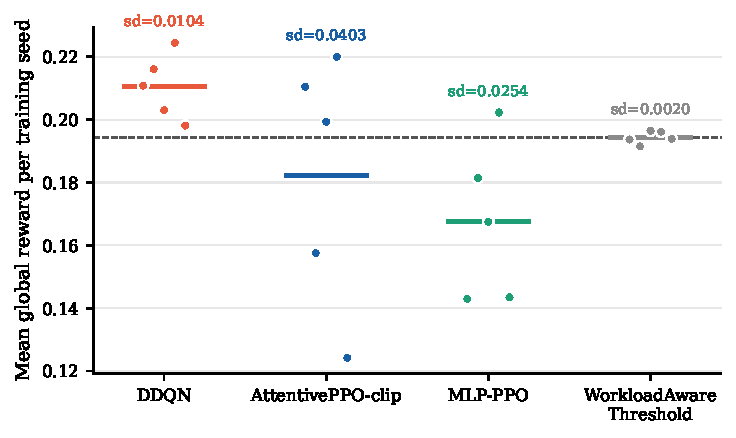
\includegraphics[width=0.72\linewidth]{charts/fig_seed_variability}
\caption{\label{fig:seedvar}\textbf{Per-seed reward: the variability a single
  checkpoint conceals.}
  Each point is the mean global reward of one independently trained
  agent (5 episodes each); the horizontal bar is the across-seed mean
  and the dashed line the best heuristic. \attentive{} spans
  0.124--0.220, so whether it appears to beat the best heuristic depends
  on which seed is evaluated. \ddqn{} is both higher and markedly more
  stable. The heuristic itself is near-deterministic
  (s.d.\ $= 0.0020$), reflecting environment noise alone.}
\end{figure}

\FloatBarrier

\subsection*{Ablation: the two specialists interact non-additively}
\label{sec:ablation}

Table~\ref{tab:ablation} isolates the contribution of each specialist by
restricting the agent to the corresponding action sub-space. We report
absolute rewards rather than percentage gains over
\texttt{PartitionOnly}, because that baseline suffers uncontrolled file
proliferation and a ratio against it is close to tautological.

The informative comparison is against \texttt{CompactOnly}. The full
agent and \texttt{CompactOnly} are physically almost identical --- 51.6
versus 48.4 mean files, 331 versus 314\,ms mean latency --- so
essentially the entire $0.0621$ reward difference is attributable to
partition pruning (0.225 versus exactly 0.000).

\texttt{PartitionOnly} establishes the interaction. Despite being the
partition specialist acting alone, its pruning ratio \emph{collapses} to
0.080, well below the 0.225 the same specialist achieves within the full
agent. Without compaction, data is never rewritten into the newly
declared partition layout, so declaring a partition specification does
not by itself deliver pruning. Compaction is thus a prerequisite for
partitioning to have any effect, and the two decisions cannot be
optimised independently.

\begin{table}[!htbp]
\centering
\begin{tabular}{lccccc}
\toprule
\textbf{Configuration} & \textbf{Reward} & $\Delta$ \textbf{vs.\ full} &
  \textbf{Pruning} & \textbf{Files} & \textbf{Latency (ms)} \\
\midrule
Full hierarchical agent    & 0.1823    & ---       & 0.225 & 51.6  & 331 \\
\texttt{CompactOnly}       & 0.1202    & $-$0.0621 & 0.000 & 48.4  & 314 \\
\texttt{PartitionOnly}     & $-$0.1099 & $-$0.2922 & 0.080 & 793.0 & 3{,}643 \\
\bottomrule
\end{tabular}
\caption{\label{tab:ablation}\textbf{Specialist ablation.}
  Each ablation restricts the agent to one specialist's action
  sub-space, holding architecture and training configuration fixed.
  Both differences from the full agent are significant
  ($p_{\text{Holm}} = 0.0022$, $|\delta| \geq 0.97$). The full agent and
  \texttt{CompactOnly} reach nearly identical physical table states, so
  their reward gap is almost entirely pruning; \texttt{PartitionOnly}
  demonstrates that partitioning without compaction does not deliver
  pruning.}
\end{table}

\begin{figure}[!htbp]
\centering
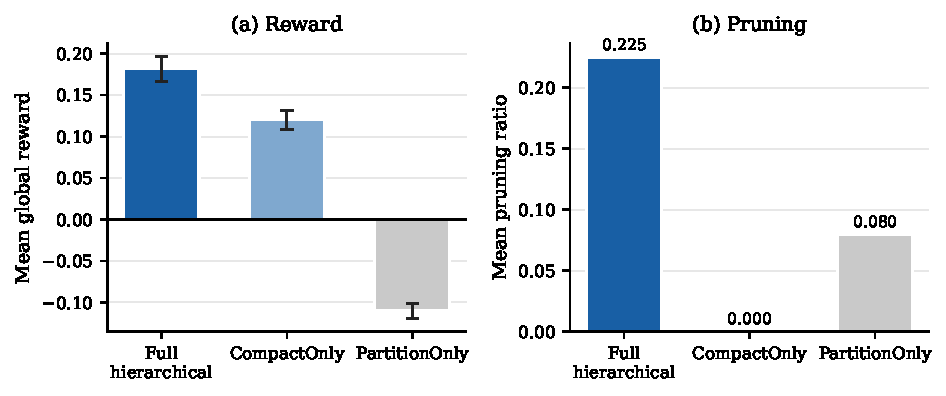
\includegraphics[width=0.82\linewidth]{charts/fig_ablation}
\caption{\label{fig:ablation}\textbf{Ablation of the two specialists.}
  \textbf{(a)}~Mean global reward with bootstrap 95\% confidence
  intervals. \textbf{(b)}~Mean partition pruning ratio.
  \texttt{PartitionOnly} attains only 0.080 pruning despite being the
  partition specialist, because without compaction the data is never
  rewritten into the declared layout --- the interaction between the two
  specialists is non-additive.}
\end{figure}

\FloatBarrier

\subsection*{Sensitivity to hand-chosen constants}
\label{sec:sensitivity}

The framework contains three sets of values chosen by hand: the
meta-controller constants, the environment's pruning matrix, and the
reward weights. We vary each in turn.

\textbf{Meta-controller constants.}
Table~\ref{tab:meta} sweeps the urgency threshold $\theta$, the
utilisation boost, and both cooldowns one at a time around the published
operating point, evaluating each configuration on the same three matched
episodes. Reward varies by 0.0295 across the entire grid, or 14.5\% of
the default configuration's value, and no configuration collapses.
The published constants are reasonable but mildly conservative: a
2-step compaction cooldown would have improved reward by 8.2\%. We note
that the two worst configurations fall slightly below the best
heuristic, so the meta-controller is robust within a sensible range
rather than universally.

\begin{table}[!htbp]
\centering
\begin{tabular}{llccc}
\toprule
\textbf{Parameter varied} & \textbf{Value} & \textbf{Reward} &
  \textbf{95\% CI} & \textbf{\% vs.\ default} \\
\midrule
\emph{(default)} & $\theta = 0.35$, boost $0.15$, $c_c = 4$, $c_p = 20$
                                & 0.2033 & [0.1941, 0.2154] & --- \\
\midrule
Urgency threshold $\theta$ & 0.25 & 0.1935 & [0.1914, 0.1947] & $-$4.8 \\
                           & 0.30 & 0.1909 & [0.1877, 0.1953] & $-$6.1 \\
                           & 0.40 & 0.2041 & [0.1927, 0.2199] & $+$0.4 \\
                           & 0.45 & 0.2019 & [0.1877, 0.2206] & $-$0.7 \\
Utilisation boost          & 0.00 & 0.1967 & [0.1871, 0.2108] & $-$3.2 \\
                           & 0.30 & 0.2071 & [0.1944, 0.2212] & $+$1.9 \\
Compaction cooldown $c_c$  & 2    & \textbf{0.2200} & [0.2048, 0.2294] & $+$\textbf{8.2} \\
                           & 8    & 0.1941 & [0.1779, 0.2050] & $-$4.5 \\
Partition cooldown $c_p$   & 10   & 0.2033 & [0.1940, 0.2194] & $+$0.0 \\
                           & 40   & 0.1905 & [0.1712, 0.2102] & $-$6.3 \\
\bottomrule
\end{tabular}
\caption{\label{tab:meta}\textbf{Meta-controller sensitivity.}
  One-at-a-time perturbation of every hand-chosen meta-controller
  constant, three matched episodes per configuration. Total spread
  across the grid is 0.0295 (14.5\% of the default). With $n = 3$ an
  exact permutation test cannot reach $p < 0.25$, so this analysis is
  powered for \emph{estimation} rather than hypothesis testing and we
  report magnitudes and intervals rather than $p$-values.}
\end{table}

\begin{figure}[!htbp]
\centering
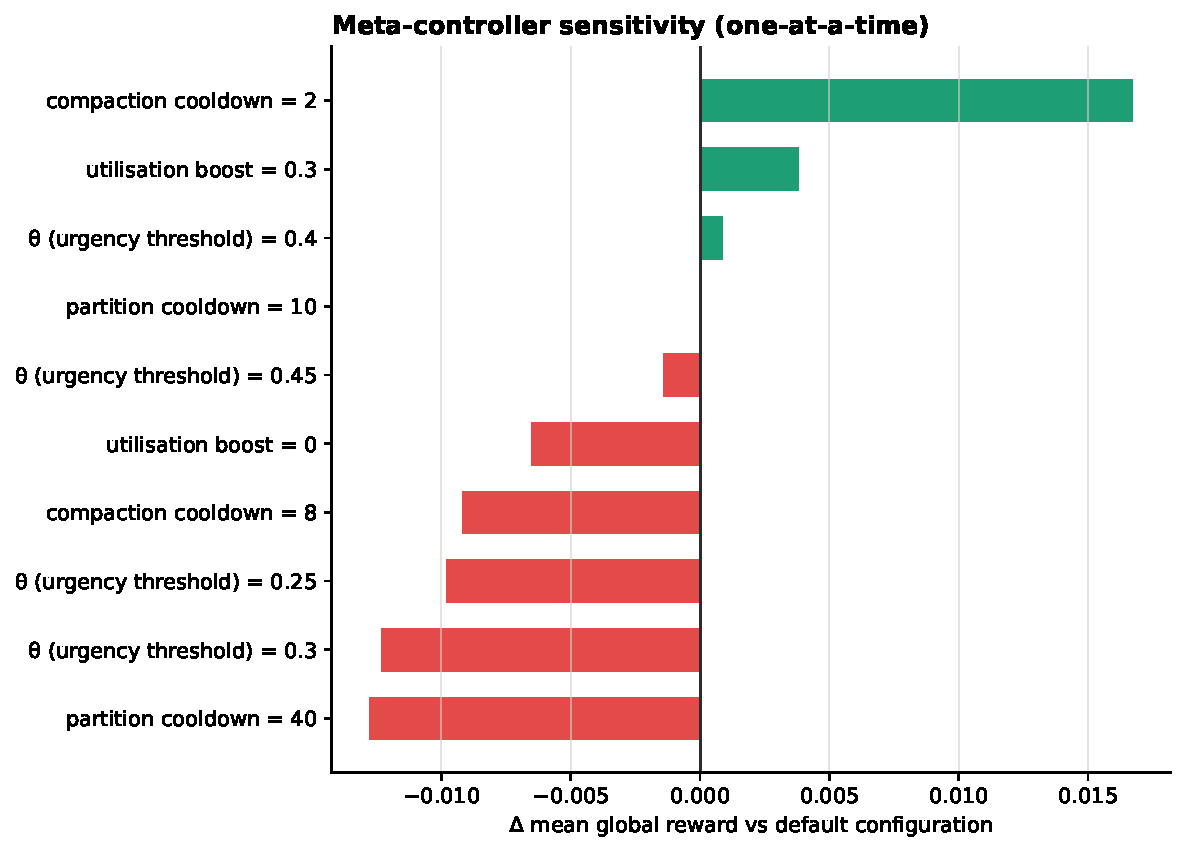
\includegraphics[width=0.78\linewidth]{charts/fig_meta_tornado}
\caption{\label{fig:tornado}\textbf{Meta-controller sensitivity (tornado plot).}
  Deviation in mean global reward from the default configuration for
  each one-at-a-time perturbation, ordered by magnitude. The compaction
  cooldown is the most influential constant; the partition cooldown and
  urgency threshold follow. No perturbation causes collapse.}
\end{figure}

\textbf{Pruning matrix.}
The environment's query benefit is driven by a lookup table mapping
(query type, partition strategy) pairs to a fraction of files skipped
(Table~\ref{tab:pruning}). These values are assumed rather than measured
--- a limitation we state plainly in the Discussion. To test whether our
conclusions depend on them, we scaled every non-zero entry by
$\{0.8, 0.9, 1.0, 1.1, 1.2\}$ and re-evaluated both the best RL agent
and the best heuristic at each scale, so that the \emph{gap} rather than
only the absolute score can be tracked (Table~\ref{tab:pruningscale}).

The RL advantage is positive at every scale, including a 20\% weaker
pruning benefit. We also note a fact that bears directly on the concern
that the advantage is an artefact of the pruning table: \ddqn{} wins
while achieving \emph{lower} pruning than the best heuristic (0.204
versus 0.248, Table~\ref{tab:ranking}). Its advantage comes from
compaction quality --- 37 files versus 50, 220\,ms versus 324\,ms ---
rather than from exploiting the pruning table more aggressively.

\begin{table}[!htbp]
\centering
\begin{tabular}{cccc}
\toprule
\textbf{Pruning scale} & \ddqn{} & \texttt{WorkloadAwareThreshold} &
  \textbf{Gap} \\
\midrule
0.8 & 0.1865 & 0.1817 & $+$0.0048 \\
0.9 & 0.1976 & 0.1882 & $+$0.0094 \\
1.0 & 0.2005 & 0.1971 & $+$0.0034 \\
1.1 & 0.2122 & 0.2015 & $+$0.0106 \\
1.2 & 0.2162 & 0.2076 & $+$0.0086 \\
\bottomrule
\end{tabular}
\caption{\label{tab:pruningscale}\textbf{Sensitivity to the pruning matrix.}
  All non-zero pruning values scaled by a common factor; both the best
  RL agent and the best heuristic re-evaluated at each scale on matched
  episodes. The RL advantage remains positive throughout, so the
  qualitative conclusion does not depend on the exact assumed values.}
\end{table}

\begin{figure}[!htbp]
\centering
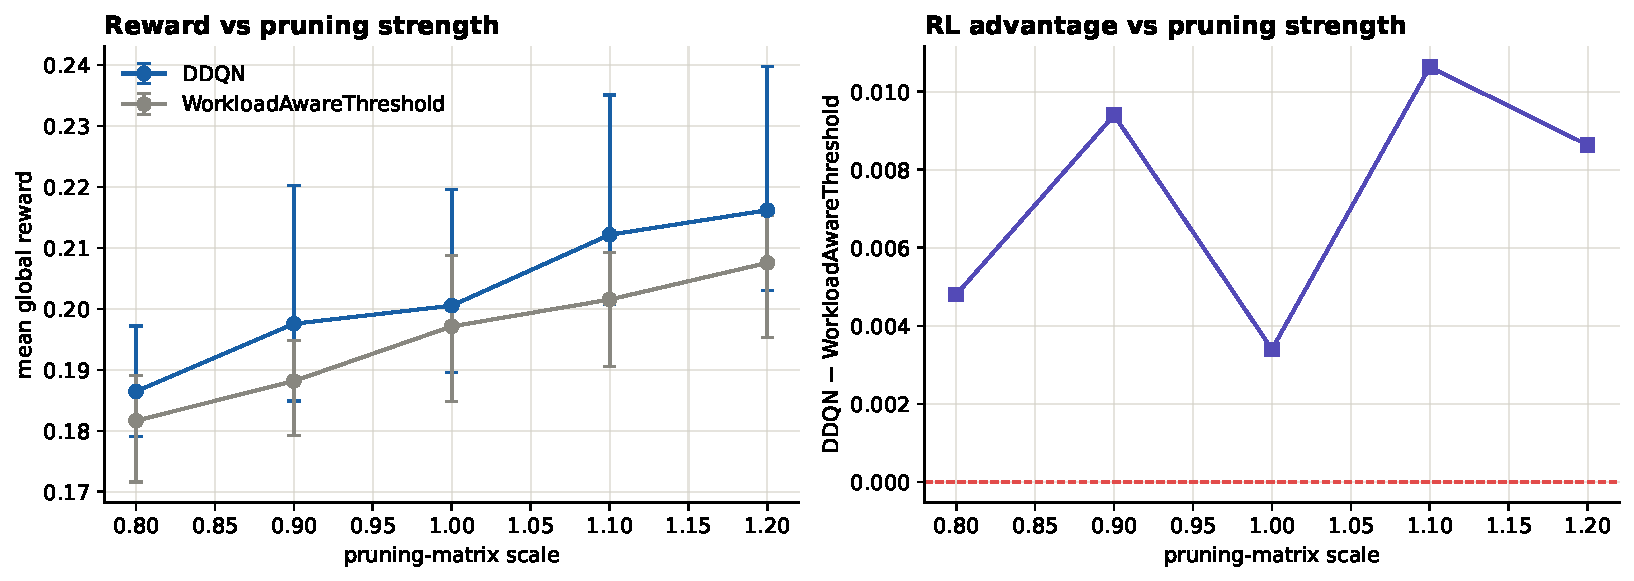
\includegraphics[width=0.70\linewidth]{charts/fig_pruning_gap}
\caption{\label{fig:pruninggap}\textbf{RL advantage under perturbation of the pruning
  matrix.}
  Mean global reward for \ddqn{} and the best heuristic as all non-zero
  pruning values are scaled by a common factor, with the gap shaded.
  Both policies improve as pruning becomes more effective, but the
  advantage of the learned policy persists at every scale.}
\end{figure}

\textbf{Reward weights and cost prices.}
Perturbing each of the four global-reward weights by $\pm$25\% and
renormalising leaves the policy ranking essentially unchanged (Spearman
$\rho \geq 0.95$ against the published weighting in all nine variants,
with \ddqn{} ranked first under every one); the changes that occur are
adjacent swaps among mid-table heuristics. Varying the three cost-model
unit prices over $\{0.5\times, 1\times, 2\times\}$ in all 27
combinations never changes the cost ordering, and neither does replacing
the flat per-operation compaction charge with a size-proportional one.

\FloatBarrier

\subsection*{An oracle meta-controller does not upper-bound the rule-based design}
\label{sec:oracle}

To quantify what the rule-based arbitration tier costs, we implemented a
greedy oracle meta-controller using environment snapshot and rollback.
At each step the world is advanced once by ingestion, a snapshot is
taken, and each of the three delegations (\noop{}, compaction
specialist, partition specialist) is executed as a trial branch with its
\emph{realised} reward measured by actually running the query. The
Iceberg data snapshot, partition specification, simulator state and both
agents' observation windows are then restored, and the best branch is
executed for real. We chose rollback over model-based lookahead because
the reward depends on measured query latency, which no model in our
system predicts accurately (a fitted predictor reaches only
$R^2 = 0.67$), so a lookahead oracle would bound the model rather than
the environment.

The result is a negative one, and informative.
\textbf{The greedy oracle scores 0.0546 against the rule-based
controller's 0.2306 --- it does not upper-bound the design at all.}
Table~\ref{tab:oracle} shows why: the per-step reward difference between
the three delegations has median 0.0069, while reward noise arising from
query-latency variation alone has $\sigma = 0.0120$. The selection
signal lies below the environment's own measurement noise, so the oracle
largely selects whichever branch happened to draw a fast query, and the
correlation between a branch's trial reward and its realised reward is
only 0.156. More fundamentally, maintenance is an investment whose
payoff is delayed; a one-step realised reward cannot observe it. The two
controllers agree on only 22.7\% of steps.

We therefore report this as evidence that \emph{when to act} is not a
greedy optimisation problem in this domain, and that the cooldowns and
urgency thresholds encode temporal structure that a myopic optimiser
cannot discover. The practical bound on the rule-based design instead
comes from Table~\ref{tab:meta}: the best configuration in the sweep
scores 0.2200 against the default's 0.2033, so the loss attributable to
suboptimal constants is approximately 8\%.

\begin{table}[!htbp]
\centering
\begin{tabular}{lc}
\toprule
\textbf{Quantity} & \textbf{Value} \\
\midrule
Rule-based meta-controller, mean global reward   & 0.2306 \\
Greedy one-step oracle, mean global reward       & 0.0546 \\
\midrule
Median per-step spread between the three branch rewards & 0.0069 \\
Reward noise from query-latency variation alone ($\sigma$) & 0.0120 \\
Correlation(trial reward, realised reward)       & 0.156 \\
Oracle gain over always-\noop{}, per step        & $+$0.00016 \\
Delegation agreement with the rule-based controller & 22.7\% \\
\bottomrule
\end{tabular}
\caption{\label{tab:oracle}\textbf{Why greedy meta-control fails.}
  The oracle selects among delegations by measured one-step reward after
  environment rollback. Because the spread between delegations is
  smaller than the environment's latency-induced reward noise, selection
  is dominated by noise rather than by signal, and the delayed payoff of
  maintenance is invisible to a one-step objective.}
\end{table}

\FloatBarrier

\subsection*{Generalization to held-out workloads}
\label{sec:generalization}

The agents are trained on trajectories from the standard workload, in
which query-profile transitions are abrupt and each phase is dominated
by a single query type. We constructed two workloads that violate these
assumptions and were never seen in training:

\begin{itemize}
\item \texttt{drift500} --- the same five profiles in the same order,
  but transitions are linear interpolations of query-type probabilities
  over 50-step windows rather than step changes.
\item \texttt{mixed500} --- each phase samples 50/50 from two profiles
  simultaneously, so no single query type dominates. This directly
  attacks the partition specialist's mechanism, since under a mixture
  there is no single correct partition specification.
\end{itemize}

Table~\ref{tab:generalization} shows that the RL advantage persists.
\ddqn{} remains the top policy on both workloads, and its margin over
the best heuristic is essentially unchanged ($+$0.0162 in distribution,
$+$0.0140 under drift, $+$0.0160 under mixture). Degradation tracks
pruning loss closely, and \texttt{AlwaysCompact\_C128} --- which never
partitions and therefore has no workload-alignment mechanism to
disrupt --- is the only policy that does not degrade, confirming that
the effect is specific to partition alignment rather than general noise.
The partition-dependent policies degrade most under mixture, as
predicted.

This design uses one episode per seed. With $n = 5$ paired observations
an exact two-sided permutation test has a minimum achievable $p$ of
0.0625, so this study is powered for estimation rather than hypothesis
testing; we report effect sizes ($\delta$ from $-0.20$ to $-0.44$) and
intervals rather than claiming significance.

\begin{table}[!htbp]
\centering
\begin{tabular}{lccccc}
\toprule
\textbf{Policy} & \textbf{Baseline} & \texttt{drift500} & $\Delta$\% &
  \texttt{mixed500} & $\Delta$\% \\
\midrule
\ddqn{}                          & 0.2105 & \textbf{0.2009} & $-$4.5  & \textbf{0.1994} & $-$5.3 \\
\texttt{WorkloadAwareThreshold}  & 0.1943 & 0.1869 & $-$3.8  & 0.1834 & $-$5.6 \\
\texttt{AlwaysCompact\_C128}     & 0.1903 & 0.1902 & $-$0.05 & 0.1898 & $-$0.2 \\
\attentive{}                     & 0.1823 & 0.1788 & $-$1.9  & 0.1638 & $-$10.2 \\
\mlpppo{}                        & 0.1675 & 0.1609 & $-$4.0  & 0.1469 & $-$12.3 \\
\bottomrule
\end{tabular}
\caption{\label{tab:generalization}\textbf{Performance on two held-out workloads.}
  \texttt{drift500} replaces abrupt profile transitions with 50-step
  linear interpolations; \texttt{mixed500} samples two profiles
  concurrently in every phase. Neither was seen during training.
  \ddqn{} remains the highest-scoring policy on both, and
  \texttt{AlwaysCompact\_C128} --- the only policy with no partitioning
  mechanism --- is the only one that does not degrade.}
\end{table}

\begin{figure}[!htbp]
\centering
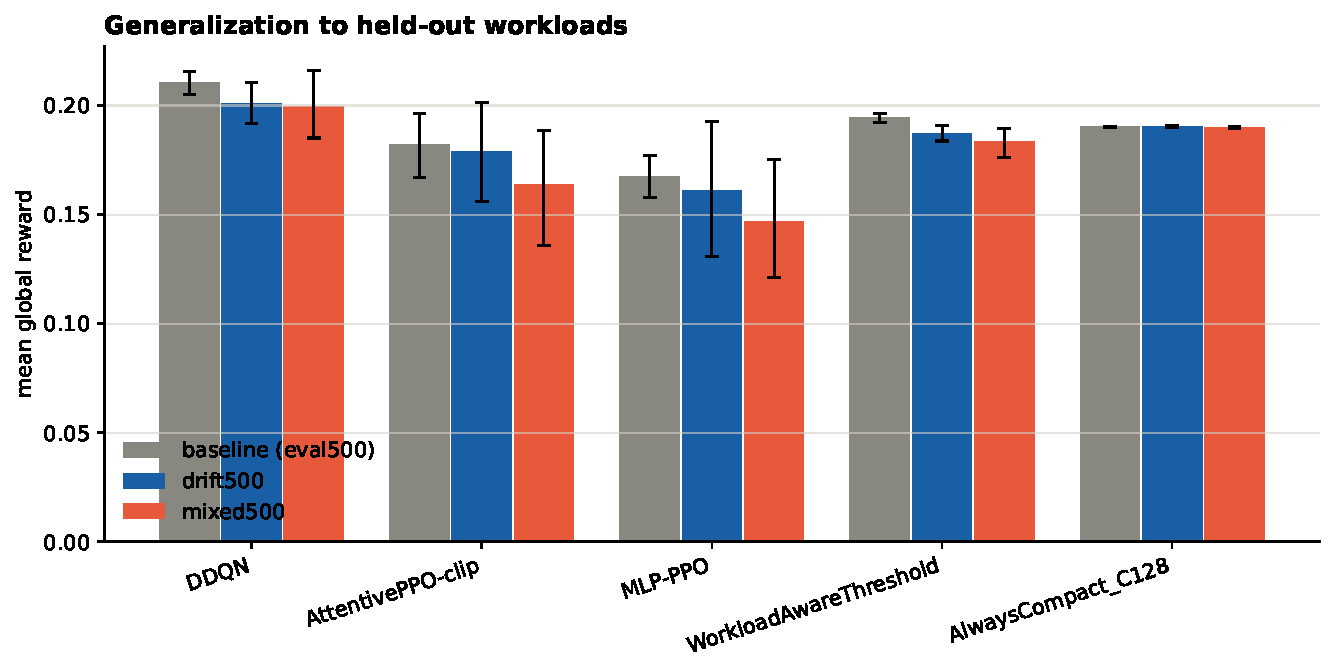
\includegraphics[width=0.86\linewidth]{charts/fig_generalization}
\caption{\label{fig:generalization}\textbf{Degradation on held-out workloads.}
  Relative change in mean global reward from the in-distribution
  baseline for each policy under drifting transitions and concurrent
  query mixtures. Policies that rely on partition alignment degrade
  most under mixture; the pure-compaction heuristic is unaffected,
  isolating the mechanism responsible.}
\end{figure}

\FloatBarrier

\subsection*{Online adaptation}
\label{sec:adaptive}

We evaluate whether continuing to update weights during deployment helps
or harms, starting each run from a frozen checkpoint and applying the
appropriate online algorithm over five consecutive 500-step episodes.

Our original submission reported that online adaptation improved
\attentive{} by $+$20.3\% while destabilising \ddqn{} by $-$22.2\%, and
drew from that contrast a general conclusion about on-policy versus
off-policy adaptation. Auditing this experiment revealed three defects,
each independently sufficient to produce the reported collapse. First,
the Double-DQN update regressed the model's softmax output rather than
its raw $Q$-values: our model returns $(\mathrm{softmax}(Q), \max Q)$
for interface uniformity, and the online update consumed the first
return value, fitting temporal-difference targets against a probability
vector bounded in $[0,1]$. Second, $\varepsilon$ was decremented once
per update call rather than once per environment step, so the
``adaptive'' agent explored at $\varepsilon \approx 1.0$ throughout.
Third, the runs were initialised from checkpoints affected by the
pipeline defects described above.

Table~\ref{tab:adaptive} reports the corrected experiment. All three
architectures are stable and every confidence interval straddles zero.
\textbf{We therefore withdraw the claim that off-policy value-based
methods destabilise under online adaptation in this environment}; it was
an implementation defect, not a property of the algorithm class. We also
did not pursue the remedies that such a collapse would motivate
(prioritised replay, shorter target-update intervals, sliding-window
buffers), because there is no collapse to rescue.

The honest reading of Table~\ref{tab:adaptive} is that over a short
deployment window adaptation is \emph{neutral}. With five 500-step
episodes each specialist receives roughly 500 transitions and 25
gradient updates, which measures fine-tuning drift rather than
substantial online learning --- which is precisely why the intervals
straddle zero.

\begin{table}[!htbp]
\centering
\begin{tabular}{lccccc}
\toprule
\textbf{Architecture} & \textbf{Ep.\ 1 $\to$ 5} & \textbf{95\% CI} &
  \textbf{Adaptive mean} & \textbf{Frozen ceiling} &
  \textbf{\% gap closed} \\
\midrule
\ddqn{}      & $+$3.8\% & [$-$4.8, $+$11.4] & 0.2092 & 0.2105 & n/a \\
\mlpppo{}    & $-$4.2\% & [$-$12.9, $+$2.4] & 0.2093 & 0.1675 & n/a \\
\attentive{} & $+$8.4\% & [$-$5.0, $+$21.9] & 0.1998 & 0.1823 & n/a \\
\bottomrule
\end{tabular}
\caption{\label{tab:adaptive}\textbf{Online adaptation over five consecutive episodes.}
  Change from the first to the fifth adaptation episode with bootstrap
  95\% confidence intervals over five seeds. All intervals straddle
  zero: adaptation neither helps nor harms materially over this window,
  and no architecture collapses. The ``\% gap closed'' metric is
  reported as \texttt{n/a} whenever the initial gap to the frozen
  ceiling is below 0.01, because the ratio is numerically unstable at
  that scale; the guard is implemented in the released analysis code
  rather than applied by hand.}
\end{table}

\begin{figure}[!htbp]
\centering
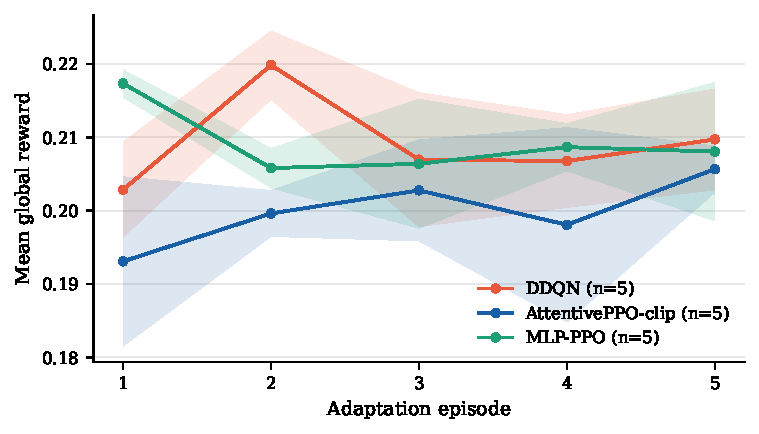
\includegraphics[width=0.74\linewidth]{charts/fig_adaptive}
\caption{\label{fig:adaptive}\textbf{Online adaptation trajectories.}
  Mean global reward per adaptation episode, averaged over five seeds
  per architecture; shaded bands are $\pm$1 standard error. Trajectories
  are flat within noise and the bands overlap throughout, supporting the
  conclusion that adaptation is neutral over a short deployment window
  for all three architectures.}
\end{figure}

\FloatBarrier

\subsection*{What the attention encoder actually does}
\label{sec:attention}

Our original submission attributed a $+$3.5\% reward advantage to the
self-attention encoder's ability to weight recent observations
differentially under workload shift. That claim was confounded and is
not supported by direct measurement.

\textbf{The comparison was confounded by capacity, in opposite
directions per specialist.} The published \mlpppo{} had 17\% \emph{fewer}
parameters than \attentive{} on the compaction specialist but 42\%
\emph{more} on the partition specialist. We therefore constructed a
parameter-matched feedforward control, \matchedmlp{}, sized to within
0.06\% of \attentive{} on each specialist separately
(Table~\ref{tab:matched}). Capacity-matched, the advantage disappears
($\Delta = 0.0049$, $p = 0.54$, $\delta = +0.16$, small).

An incidental finding is that \matchedmlp{} \emph{outperforms} the
published \mlpppo{} (0.1774 versus 0.1675) while using fewer total
parameters, because the published model's capacity was mis-allocated
between the two specialists. Part of the originally reported gap was
therefore architecture \emph{sizing} rather than architecture family.

\begin{table}[!htbp]
\centering
\begin{tabular}{lccc}
\toprule
\textbf{Model} & \textbf{Reward} & \textbf{95\% CI} & \textbf{Params} \\
\midrule
\attentive{}  & 0.1823 & [0.1669, 0.1963] & 170{,}571 \\
\matchedmlp{} & 0.1774 & [0.1664, 0.1885] & 170{,}667 \\
\mlpppo{} (published sizing) & 0.1675 & [0.1579, 0.1772] & 192{,}203 \\
\bottomrule
\end{tabular}
\caption{\label{tab:matched}\textbf{Capacity-matched attention control.}
  \matchedmlp{} is a feedforward network sized to within 0.06\% of
  \attentive{} on each specialist. The difference between \attentive{}
  and \matchedmlp{} is not significant ($p = 0.54$, Cliff's
  $\delta = +0.16$), so the previously reported attention advantage does
  not survive capacity matching.}
\end{table}

\begin{figure}[!htbp]
\centering
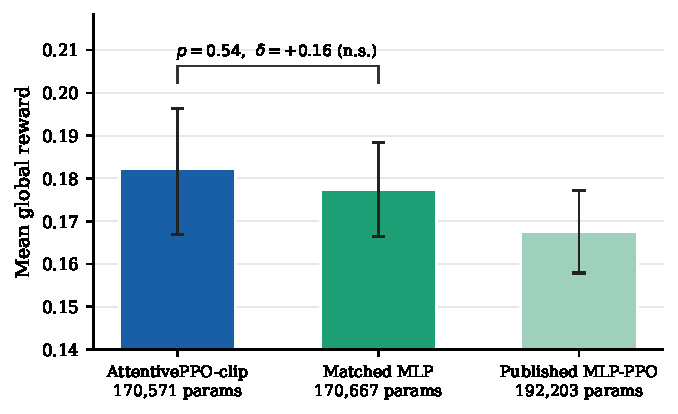
\includegraphics[width=0.62\linewidth]{charts/fig_matched_mlp}
\caption{\label{fig:matched}\textbf{Attention versus a parameter-matched feedforward
  control.}
  Mean global reward with bootstrap 95\% confidence intervals. Matching
  capacity to within 0.06\% eliminates the previously reported
  attention advantage. The published \mlpppo{} underperforms both,
  reflecting mis-allocated capacity between the two specialists rather
  than a property of feedforward encoders.}
\end{figure}

\textbf{Direct measurement of the attention weights.}
We captured multi-head attention scores at every step of frozen
1{,}000-step rollouts across three seeds
(Table~\ref{tab:attnprofile}, Fig.~\ref{fig:attnprofile}). The partition
specialist places 51.7\% of its attention mass on the single most recent
timestep of a 20-step window (uniform would be 5.0\%), while the
compaction specialist is only $1.29\times$ uniform --- close enough to
flat that the global average pooling which follows performs a similar
function.

Attention concentrated on one position is a \emph{recency gate}, not
sequence modelling. Furthermore, if the encoder were exploiting workload
structure, its focus should shift at profile transitions. It does not:
around the four transitions the change in recency mass is negligible and
inconsistent in direction across seeds ($\Delta = -0.0066$ for
compaction, $+0.0031$ for partition; Fig.~\ref{fig:attntrans}).

\begin{table}[!htbp]
\centering
\begin{tabular}{lccccc}
\toprule
\textbf{Specialist} & \textbf{Uniform} & \textbf{Newest} &
  \textbf{$-$1} & \textbf{$-$2} & \textbf{$-$3} \\
\midrule
Compaction ($W = 10$) & 0.100 & 0.150 & 0.125 & 0.113 & 0.102 \\
Partition ($W = 20$)  & 0.050 & \textbf{0.517} & 0.105 & 0.051 & 0.032 \\
\bottomrule
\end{tabular}
\caption{\label{tab:attnprofile}\textbf{Attention mass by position.}
  Mean attention mass assigned to the most recent timesteps of the
  observation window, averaged over three seeds and 1{,}000 steps each.
  The partition specialist concentrates over half its attention on a
  single position; the compaction specialist is only $1.29\times$
  uniform. Neither profile changes meaningfully at workload
  transitions.}
\end{table}

\begin{figure}[!htbp]
\centering
\begin{subfigure}[t]{0.48\textwidth}
  \centering
  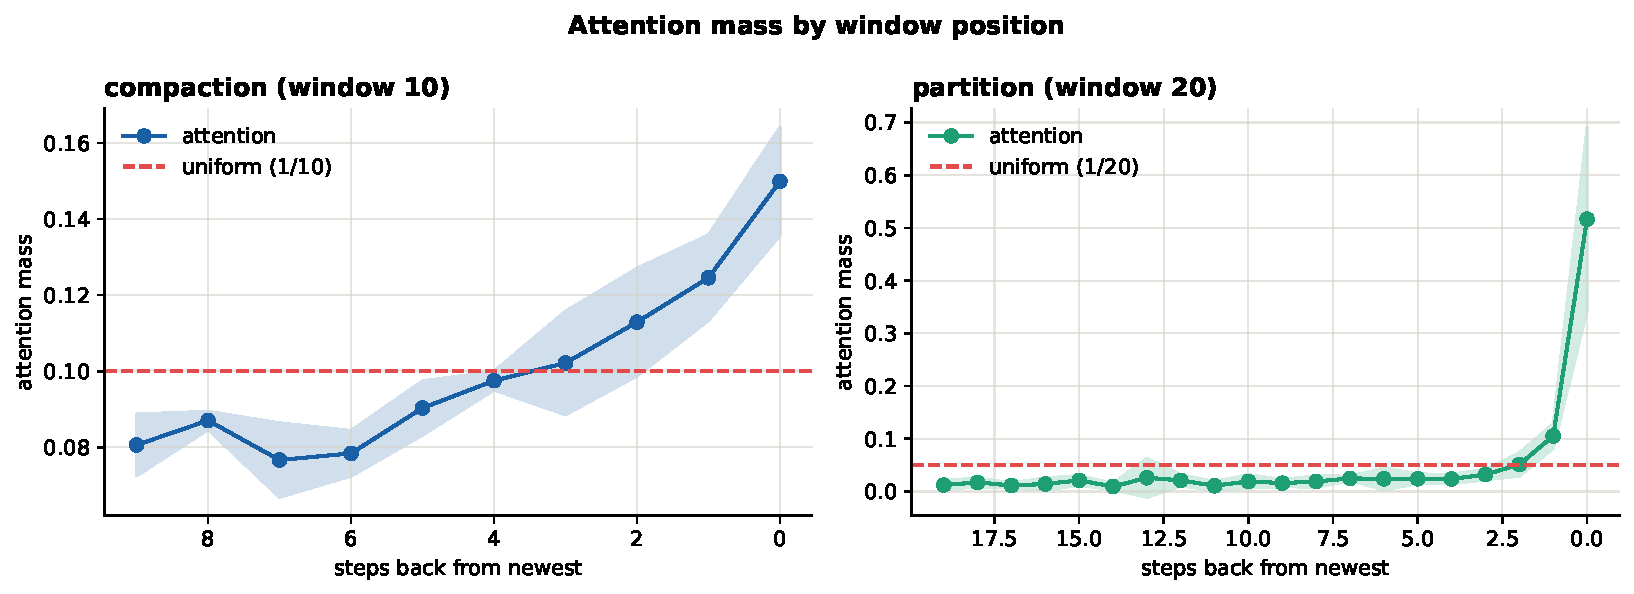
\includegraphics[width=\linewidth]{charts/fig_attention_profile}
  \caption{\textbf{Attention mass by window position.}
  Both specialists exhibit a monotone recency profile with no structure
  beyond the most recent steps.}
  \label{fig:attnprofile}
\end{subfigure}
\hfill
\begin{subfigure}[t]{0.48\textwidth}
  \centering
  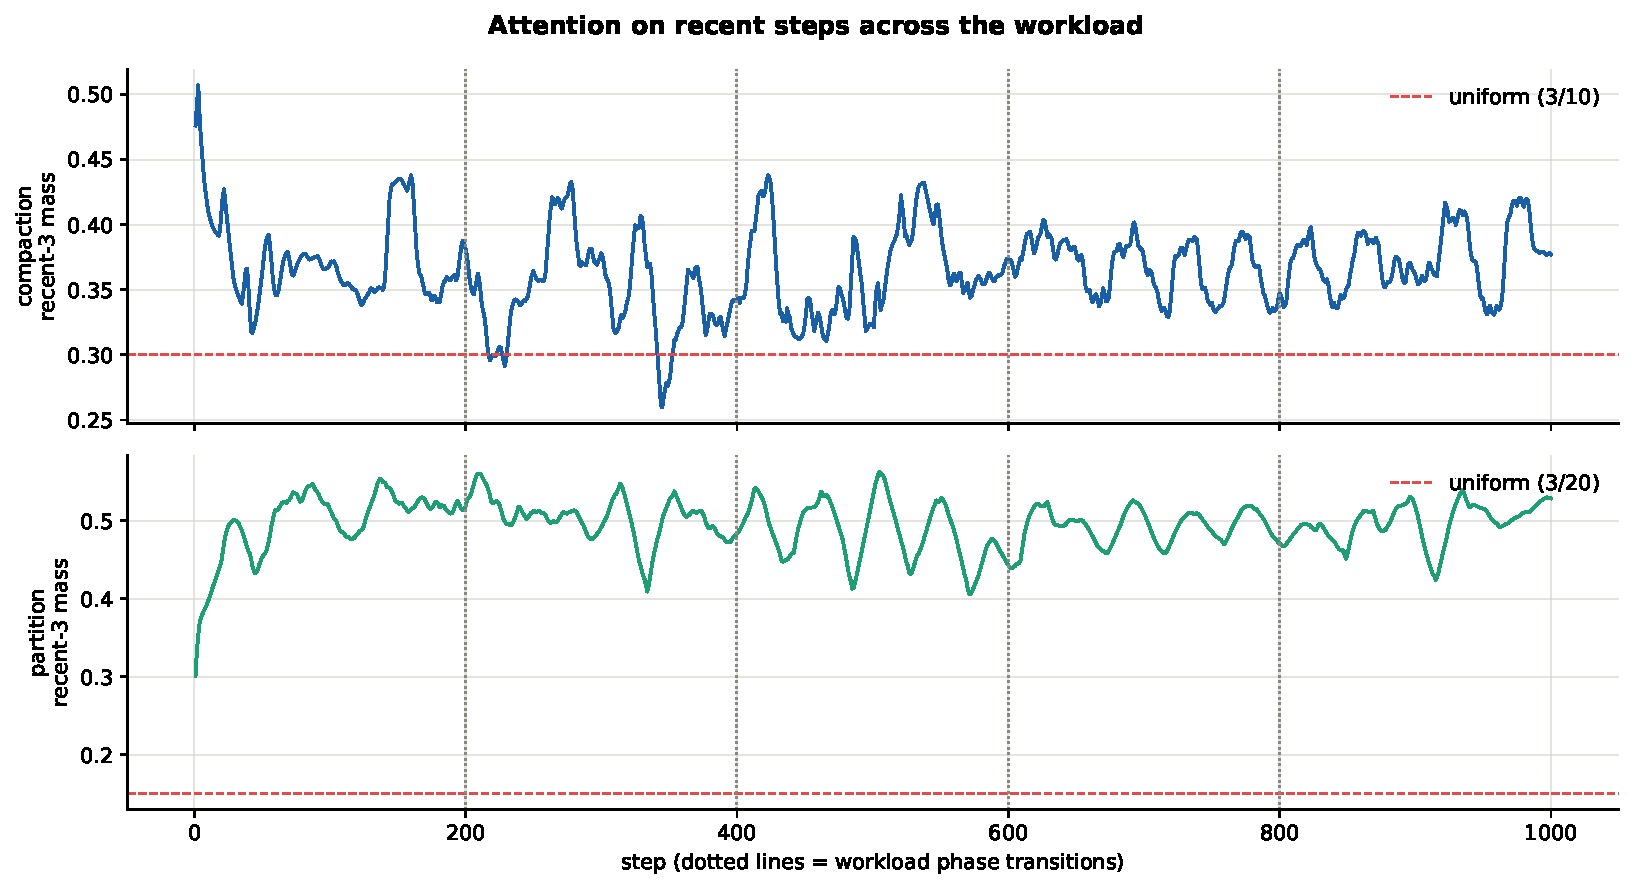
\includegraphics[width=\linewidth]{charts/fig_attention_transitions}
  \caption{\textbf{Recency mass at workload transitions.}
  Change in recency focus around the four profile transitions is
  negligible and inconsistent in sign across seeds.}
  \label{fig:attntrans}
\end{subfigure}
\caption{\textbf{The attention encoder behaves as a static recency gate.}
  Attention scores captured at every step of frozen 1{,}000-step
  rollouts across three seeds.}
\label{fig:attention}
\end{figure}

Three further observations are coherent with this interpretation and are
reported in full in the supplementary sweep. A feedforward network can
express a fixed positional weighting, which explains the
capacity-matched tie. Increasing the encoder to $7\times$ the parameters
changes nothing (0.1830), so the mechanism is not capacity-limited.
Doubling the context window \emph{hurts} (0.1765), because extending a
static profile only adds diluting positions.

\textbf{Exploratory tuning.}
We additionally asked whether attention improves under a configuration
better suited to it. Of the variants tested, only a longer training
budget helped, and only modestly: $+$0.0058 ($p = 0.11$, not
significant), reaching parity with the best heuristic (0.1949 versus
0.1943) but remaining below \ddqn{}. We state explicitly that \ddqn{}
was \emph{not} given an equivalent tuning sweep, so this result means
that attention can be brought closer with tuning, not that the
architectures are equivalent under equal tuning effort. This study is
exploratory and is deliberately separated from the matched-configuration
comparison in Table~\ref{tab:threeway}.

\FloatBarrier

\subsection*{Computational cost}
\label{sec:cost}

Table~\ref{tab:inference} reports per-step inference latency measured
over 10{,}000 randomised observations on CPU only. The rule-based
meta-controller costs approximately 2\,$\mu$s and is effectively free.
Notably, \attentive{} is $3\times$ slower than \mlpppo{} despite having
\emph{fewer} parameters, because self-attention is quadratic in window
length --- a deployment consideration that parameter counts do not
reveal.

\begin{table}[!htbp]
\centering
\begin{tabular}{lccc}
\toprule
\textbf{Component} & \textbf{Median} & \textbf{p95} & \textbf{Params} \\
\midrule
Meta-controller (rule-based urgency) & \textbf{0.0019\,ms} & 0.003\,ms & --- \\
\mlpppo{} --- full hierarchical step   & 3.48\,ms  & 4.06\,ms  & 192{,}203 \\
\ddqn{} --- full hierarchical step     & 4.80\,ms  & 6.28\,ms  & 193{,}739 \\
\attentive{} --- full hierarchical step & 10.73\,ms & 12.57\,ms & 170{,}571 \\
\bottomrule
\end{tabular}
\caption{\label{tab:inference}\textbf{Per-step inference latency.}
  Measured over 10{,}000 randomised observations on an Intel i7-1165G7
  with no GPU present. A full hierarchical step comprises the
  meta-controller decision plus one specialist forward pass. At
  $\sim$5\,ms against a mean query latency of $\sim$344\,ms, policy
  inference costs approximately 1.4\% of a single query.}
\end{table}

Training is inexpensive in absolute terms (Table~\ref{tab:training}).
We report hardware per row because wall-clock is not comparable across
hardware; the deployed \attentive{} variant was trained on CPU.

\begin{table}[!htbp]
\centering
\begin{tabular}{llccc}
\toprule
\textbf{Variant} & \textbf{Hardware} & \textbf{Params} &
  \textbf{Per agent} & \textbf{All 5 seeds} \\
\midrule
\ddqn{}       & Tesla T4  & 193{,}739 & 2.26\,min & 11.3\,min \\
\mlpppo{}     & Tesla T4  & 192{,}203 & 1.73\,min & \phantom{0}8.7\,min \\
\attentive{}  & local CPU & 170{,}571 & 3.30\,min & 16.5\,min \\
\bottomrule
\end{tabular}
\caption{\label{tab:training}\textbf{Offline training cost per deployable agent.}
  A deployable agent comprises both specialists. Wall-clock is the mean
  over five seeds. Hardware differs by variant and wall-clock is
  therefore \emph{not} comparable across rows; we report it per row
  rather than normalising.}
\end{table}

Table~\ref{tab:cost} regenerates the cost model with the RL
infrastructure term included, so that the comparison with heuristics is
like-for-like. Inference is charged at \$0.096/h CPU and offline
training at \$0.526/h GPU amortised over 100 deployment episodes.

The saving relative to no maintenance survives: $-$82.4\% for \ddqn{},
against $-$82.9\% claimed originally, and the RL infrastructure term is
0.003\% of the total. \textbf{However, RL is not the cheapest policy.}
\texttt{Threshold10\_C128} costs less (\$8.37 versus \$8.79) because it
performs fewer compactions (124 versus 173 per episode). Under this cost
model no RL agent repays its training cost relative to that heuristic.
Reinforcement learning buys reward --- better pruning, lower latency,
and robustness to workload shift --- not minimum dollar cost, and we
state this plainly rather than presenting cost as a further advantage.

\begin{table}[!htbp]
\centering
\setlength{\tabcolsep}{4.5pt}
\begin{tabular}{lcccccrc}
\toprule
\textbf{Policy} & \textbf{Query} & \textbf{Compact} & \textbf{Storage} &
  \textbf{Inference} & \textbf{Training} & \textbf{Total} &
  \textbf{vs.\ no-maint.} \\
\midrule
\texttt{Threshold10\_C128}      & 3.31  & 0.62 & 4.45 & ---    & ---    & \textbf{8.37}  & $-$83.2\% \\
\textbf{\ddqn{}}                & 3.44  & 0.87 & 4.49 & 0.0001 & 0.0002 & \textbf{8.79}  & $-$82.4\% \\
\attentive{}                    & 4.98  & 0.82 & 4.57 & 0.0003 & 0.0003 & 10.37 & $-$79.2\% \\
\texttt{Threshold10\_C64}       & 5.71  & 0.62 & 4.57 & ---    & ---    & 10.90 & $-$78.1\% \\
\texttt{WorkloadAwareThreshold} & 5.73  & 1.05 & 4.57 & ---    & ---    & 11.35 & $-$77.2\% \\
\mlpppo{}                       & 6.37  & 0.58 & 4.67 & 0.0001 & 0.0002 & 11.62 & $-$76.7\% \\
\texttt{AlwaysCompact\_C128}    & 3.48  & 5.00 & 4.43 & ---    & ---    & 12.92 & $-$74.1\% \\
\texttt{No\_Maintenance}        & 42.98 & 0.00 & 6.88 & ---    & ---    & 49.86 & \phantom{$-$}0\% \\
\bottomrule
\end{tabular}
\caption{\label{tab:cost}\textbf{Estimated cloud cost per 1{,}000-step episode (USD).}
  Operational terms use the cost model in Methods; the inference and
  training columns are new and make the comparison with heuristics
  like-for-like. The RL infrastructure term is 0.003\% of the total for
  \ddqn{}. Note that the cheapest policy is a heuristic, not an RL
  agent.}
\end{table}

\begin{figure}[!htbp]
\centering
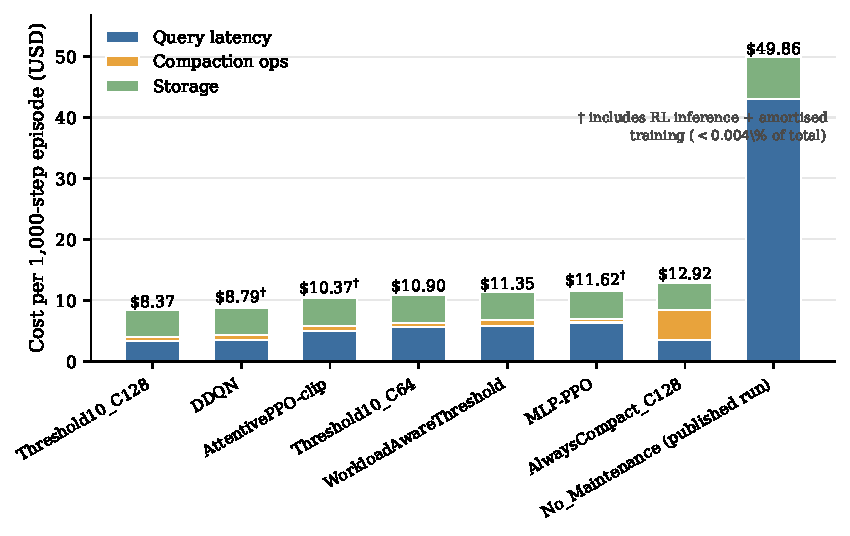
\includegraphics[width=0.86\linewidth]{charts/fig_cost}
\caption{\label{fig:cost}\textbf{Cost decomposition per 1{,}000-step episode.}
  Stacked bars show query, compaction and storage cost.
  \texttt{No\_Maintenance} is dominated by query cost from scanning
  thousands of small files; \texttt{AlwaysCompact\_C128} is dominated by
  compaction cost. Policies marked $\dagger$ additionally carry RL
  inference and amortised training cost, which is under 0.004\% of the
  total and not visible at this scale.}
\end{figure}

\FloatBarrier

% ════════════════════════════════════════════════════════════════════════════
\section*{Discussion}
\label{sec:discussion}
% ════════════════════════════════════════════════════════════════════════════

\textbf{Joint control is necessary, and the interaction is
non-additive.}
The ablation in Table~\ref{tab:ablation} shows that partitioning without
compaction does not deliver pruning: the partition specialist acting
alone reaches only 0.080 pruning against the 0.225 the same specialist
achieves within the full agent, because data is never rewritten into the
declared layout. This is the clearest architectural argument in the
paper, and it has a direct implication for system design: an
auto-optimisation subsystem that triggers compaction and clustering
independently, on separate thresholds, cannot exploit this interaction.

\textbf{Which architecture wins is determined by the training objective,
not the encoder.}
Under a matched configuration, \ddqn{} significantly outperforms both
actor-critic variants, while \attentive{} and \mlpppo{} --- which share
an objective and differ only in encoder --- are statistically
indistinguishable. Capacity-matched, the attention encoder confers no
significant advantage, and direct inspection shows it behaves as a
static recency gate that does not react to the workload transitions it
was supposed to detect. We therefore do not present these three
architectures as a ranking to be generalised. They are three
instantiations evaluated under one configuration, and we report where
they differ, where they do not, and what mechanism explains it.

\textbf{Training-run variability is a first-class result.}
The across-seed standard deviation differs fourfold between
architectures, and for \attentive{} the range spans whether or not the
agent beats the best heuristic. In a domain where a single evaluation
episode costs several minutes of real Spark execution, the temptation to
evaluate one checkpoint is strong; our own original submission did
exactly that. Figure~\ref{fig:seedvar} is the direct evidence that this
is not sufficient.

\textbf{Greedy meta-control fails for a measurable reason.}
The oracle experiment (Table~\ref{tab:oracle}) is a negative result we
consider transferable. When the per-step difference between candidate
actions is smaller than the environment's own measurement noise, a
greedy selector optimises noise. In such settings the value of a
rule-based arbitrator is not that it approximates the greedy optimum but
that its cooldowns encode temporal structure --- the delayed payoff of
maintenance --- which a one-step objective cannot represent.

\textbf{Trajectory-identity leakage in offline RL on operational logs.}
The leakage described in the Corrections subsection is, we believe, the
most broadly applicable finding here. Any feature that counts time since
an event will encode the identity of the behaviour policy that generated
the trajectory whenever logs are pooled across policies with different
action frequencies. Advantage-weighted regression and related
behaviour-cloning objectives will exploit that shortcut in preference to
the state features one intends them to learn. Detecting it requires a
counterfactual probe --- holding the state fixed and varying only the
suspect feature --- rather than any aggregate validation metric.

\textbf{Relationship to commercial auto-optimisation.}
A direct empirical comparison with Databricks, Snowflake or BigQuery
auto-optimisation is not possible: the optimisers are proprietary and
inseparable from their execution engines, and cannot be reproduced
against our environment. We restrict ourselves to a qualitative
architectural comparison based on publicly documented behaviour, and we
make no performance claim. Commercial auto-optimisation is predominantly
threshold- and statistics-driven, triggering on file-size and file-count
targets and, for clustering, on measured deviation from a target
ordering. Our contribution is not a better threshold but the framing of
maintenance as a sequential decision problem under a single objective.
Two structural differences follow. First, file management and clustering
are typically maintained as separate subsystems with independent
triggers, which the ablation above suggests forgoes a non-additive
interaction. Second, these systems reorganise data within a fixed
physical scheme, whereas our action space includes evolving the
partition specification itself. Conversely, commercial systems optimise
a robust proxy (file size, clustering depth), whereas we optimise a
composite reward whose weights we must justify --- a strength in
expressiveness and a weakness in that the weights are a design choice.
An empirical comparison would require running an identical workload on
each platform and remains valuable future work.

\textbf{When is RL worth it?}
We think the honest recommendation is conditional. Under our own cost
model a well-chosen heuristic is cheaper (\$8.37 versus \$8.79) and far
simpler, and for a static workload \texttt{AlwaysCompact\_C128} or
\texttt{Threshold10\_C128} is a strong choice; we say so explicitly. The
learned policy earns its complexity when the workload \emph{shifts},
which is where partition alignment matters and where
Table~\ref{tab:generalization} shows the advantage persisting. The
overhead of the learned policy itself is small: agents act on fewer than
24\% of steps, and the cost of deciding not to act is $\sim$5\,ms
against $\sim$344\,ms of query latency. Idleness is the correct
behaviour rather than wasted computation.

\textbf{Extensibility of the action space.}
Finer-grained maintenance actions --- Z-ordering, per-partition file-size
targets, partial compaction --- raise a combinatorial concern. We argue
the hierarchy is the mechanism that contains it: because specialists own
disjoint sub-spaces, adding a Z-ordering specialist adds one delegation
target and one action set, so growth is additive in the number of
specialists rather than multiplicative. Within a specialist, finer
granularity is better served by continuous control than by enumeration;
our discrete $\{32, 64, 128\}$\,KB targets are a coarse discretisation
of a continuous quantity, and target choice demonstrably matters. Partial
compaction is the genuinely hard case, since selecting a subset of files
is combinatorial in the number of files; we suggest it is better
expressed as a parameterised action (a predicate over file size and age)
than as a set-valued action. These are design arguments, not results.

\textbf{Limitations.}
We state the following plainly.
\emph{(i)~Scale.} \env{} is backed by a real Iceberg table on real
Spark with genuine Parquet files, genuine compaction, genuine partition
evolution and \emph{measured} query latency, but the tables reach only
4--5\,MB. At this scale latency is dominated by per-file overhead rather
than data volume, so the latency--file-count relationship is likely
steeper than in production. External validity to production-scale
deployments is untested.
\emph{(ii)~The pruning matrix is assumed, not measured.} We tested
sensitivity to it (Table~\ref{tab:pruningscale}) and the conclusions
hold, but we did not instrument Spark's scan metrics to measure
files-skipped per query. Doing so is the correct resolution and is
required future work.
\emph{(iii)~Train/evaluate objective mismatch.} Specialists are trained
on \texttt{compact\_reward} and \texttt{partition\_reward} but evaluated
on \texttt{global\_reward}, and these are not aligned in one specific
respect: the compaction reward's target-size bonus favours
\cthirtytwo{} at low ingestion, whereas measured global reward strongly
favours larger targets. This is not hypothetical --- our \mlpppo{} agent
selected \cthirtytwo{} for 99 of its 103 compactions, a direct
consequence of the mismatch and a probable contributor to its
underperformance. We report this as a design flaw in the reward
decomposition.
\emph{(iv)~Statistical power.} The sensitivity sweep ($n=3$ per
configuration) and the generalization study ($n=5$) are powered for
estimation rather than hypothesis testing, with permutation-test floors
of $p = 0.25$ and $p = 0.0625$ respectively. We report intervals and
effect sizes for these and reserve significance claims for the main
comparison.
\emph{(v)~Unequal tuning effort.} The attention tuning study has no
counterpart for \ddqn{}, so it establishes that attention can be brought
closer with tuning, not that the architectures are equivalent under
equal effort.
\emph{(vi)~Schema.} All experiments use a single table schema. The
compaction signal is schema-independent and should transfer; the
partition signal depends on the cardinality of the partitioning column,
so a substantially different schema would change achievable pruning.
This is argued, not demonstrated.
\emph{(vii)~Short adaptation window.} The online experiments span five
episodes and roughly 25 gradient updates per specialist, which measures
fine-tuning drift rather than substantial online learning.

\FloatBarrier

% ════════════════════════════════════════════════════════════════════════════
\section*{Methods}
\label{sec:methods}
% ════════════════════════════════════════════════════════════════════════════

\subsection*{The LakeGym v5 environment}

\env{} simulates a production data lakehouse backed by a real Apache
Iceberg table managed via PySpark, with an Iceberg REST catalog and
S3-compatible object storage. Each discrete time step executes:
(i)~ingest a batch of rows into the Iceberg table,
(ii)~the active policy selects one of eight discrete actions,
(iii)~a query is drawn from the current workload profile and executed
against the table, (iv)~three reward signals are computed from the
resulting table state and the \emph{measured} query latency, and
(v)~an observation vector is constructed.

We emphasise the boundary between what is real and what is simulated.
Real: the Iceberg table, the Parquet files, the
\texttt{rewrite\_data\_files} compaction, partition-spec evolution, and
query latency, which is measured by executing the query. Simulated: the
data, which is synthetic; the query set, which comprises five templates;
the scale, which reaches 4--5\,MB rather than production volumes; and
the pruning benefit, which is applied from the assumed matrix in
Table~\ref{tab:pruning} rather than measured from scan metrics.

\textbf{Table schema.}
The table contains eight columns: \texttt{device\_id} (string),
\texttt{timestamp} (timestamp), \texttt{temperature} (double),
\texttt{humidity} (double), \texttt{region} (string),
\texttt{event\_type} (string), \texttt{sensor\_value} (double),
and \texttt{payload} (string, length~100). Each row occupies
approximately 200~bytes; the default target file size is 64\,KB,
corresponding to roughly 50~rows per Parquet file.

\textbf{Action space.}
The joint action space consists of eight discrete actions
(Table~\ref{tab:actions}). Compaction actions rewrite small files into
consolidated Parquet files of the specified target size; partition
actions change the Iceberg partition specification; \noop{} takes no
maintenance action.

\begin{table}[!htbp]
\centering
\begin{tabular}{lcc}
\toprule
\textbf{Action} & \textbf{Type} & \textbf{Cost} \\
\midrule
\texttt{NOOP}                   & ---        & 0.0 \\
\texttt{COMPACT\_32KB}          & Compaction & 0.9 \\
\texttt{COMPACT\_64KB}          & Compaction & 1.0 \\
\texttt{COMPACT\_128KB}         & Compaction & 1.1 \\
\texttt{PARTITION\_HOUR}        & Partition  & 2.0 \\
\texttt{PARTITION\_REGION}      & Partition  & 2.0 \\
\texttt{PARTITION\_EVENT\_TYPE} & Partition  & 2.0 \\
\texttt{REMOVE\_PARTITION}      & Partition  & 0.7 \\
\bottomrule
\end{tabular}
\caption{\label{tab:actions}\textbf{Action space.}
  All eight discrete actions available to the joint agent with their
  associated normalised cost used in the reward function.}
\end{table}

\textbf{Observation space.}
The observation at step $t$ includes: file count $f_t$, block
utilisation $u_t$, rows ingested $r_t$, partition pruning ratio $p_t$,
running average pruning ratio $\bar{p}_t$, partition skew $s_t$, query
latency $\ell_t$, query-type history fractions (five values), steps
since last compaction $\delta_c$, and steps since last partition change
$\delta_p$. Following the correction described in Results, both
staleness features are capped and all features are normalised with
constants shared between training and serving.

\textbf{Workload plans.}
The v5 standard workload runs for 1{,}000 steps divided into five equal
query-profile phases of 199~steps each
(\texttt{time\_heavy}\,$\to$\,\texttt{region\_heavy}\,$\to$\,\texttt{mixed}\,$\to$\,\texttt{type\_heavy}\,$\to$\,\texttt{scan\_heavy}).
Each profile specifies query-type probabilities over five templates
(Table~\ref{tab:profiles}). Ingestion rate follows six phases:
warm-up (40~rows/step, steps 1--100), normal load (75, steps 101--300),
burst (225, steps 301--500), recovery (55, steps 501--700),
normal load 2 (75, steps 701--900), and wind-down (35, steps 901--1{,}000).
The v5 evaluation workload is a 2$\times$-compressed 500-step version.
Figure~\ref{fig:workload} illustrates the schedule.

The two held-out workloads used in Section~\ref{sec:generalization}
extend this specification. \texttt{drift500} replaces abrupt profile
transitions with linear interpolation of query-type probabilities over
50-step windows; \texttt{mixed500} samples each step from a 50/50
mixture of two profiles. Both are expressed as additional fields in the
workload plan and are backward compatible with the standard plan.

\begin{table}[!htbp]
\centering
\begin{tabular}{lccccc}
\toprule
\textbf{Profile} & \textbf{Time range} & \textbf{Region filter} &
  \textbf{Sensor lookup} & \textbf{Type filter} & \textbf{Full scan} \\
\midrule
\texttt{time\_heavy}   & \textbf{0.60} & 0.10 & 0.10 & 0.10 & 0.10 \\
\texttt{region\_heavy} & 0.10 & \textbf{0.60} & 0.10 & 0.10 & 0.10 \\
\texttt{mixed}         & 0.20 & 0.20          & 0.20 & 0.20 & 0.20 \\
\texttt{type\_heavy}   & 0.10 & 0.10          & 0.10 & \textbf{0.60} & 0.10 \\
\texttt{scan\_heavy}   & 0.10 & 0.10          & 0.10 & 0.10 & \textbf{0.60} \\
\bottomrule
\end{tabular}
\caption{\label{tab:profiles}\textbf{Query workload profiles.}
  Each profile specifies the sampling probability for each of five query
  templates. The dominant query type is shown in bold for focused
  profiles.}
\end{table}

\begin{figure}[!ht]
  \centering
  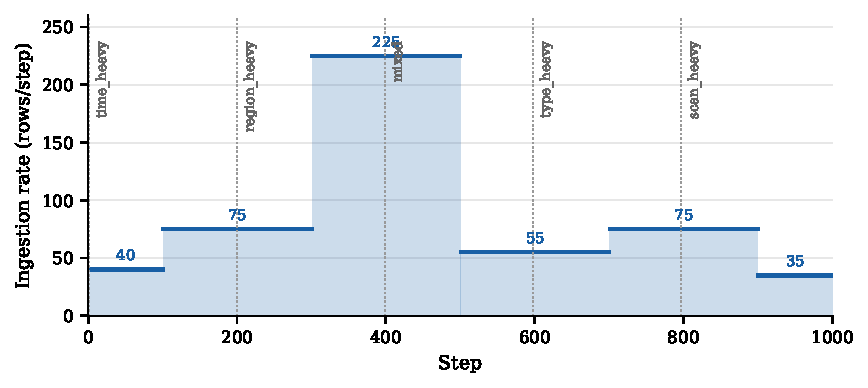
\includegraphics[width=0.85\textwidth]{charts/fig_workload_ingestion}
  \caption{\label{fig:workload}\textbf{Workload schedule for the 1{,}000-step standard plan.}
  Step function shows the ingestion rate (rows/step) across six phases,
  peaking at 225 rows/step during the burst window. Dotted vertical
  lines mark the five query-profile boundaries, which are independent of
  the ingestion phases so that storage pressure and query-mix shift are
  not confounded.}
\end{figure}

\FloatBarrier

\textbf{Pruning matrix.}
File pruning at query time is applied from a lookup table indexed by
(query type, partition strategy) (Table~\ref{tab:pruning}).
\texttt{TIME\_RANGE} queries prune 92\% of files when
\texttt{HOUR}-partitioned; \texttt{FULL\_SCAN} is irreducible under all
strategies. \textbf{These values are design assumptions, chosen to
reflect the semantic alignment between predicate and partition key.
They were not measured from Spark scan metrics.} We report a sensitivity
analysis over them in Table~\ref{tab:pruningscale} and identify their
empirical measurement as required future work.

\begin{table}[!htbp]
\centering
\begin{tabular}{lcccc}
\toprule
\textbf{Query type} & \textbf{Hour} & \textbf{Region} &
  \textbf{Event type} & \textbf{None} \\
\midrule
Time range    & \textbf{0.92} & ---           & ---           & --- \\
Sensor lookup & \textbf{0.75} & ---           & ---           & --- \\
Region filter & ---           & \textbf{0.67} & ---           & --- \\
Type filter   & ---           & ---           & \textbf{0.67} & --- \\
Full scan     & ---           & ---           & ---           & --- \\
\bottomrule
\end{tabular}
\caption{\label{tab:pruning}\textbf{Partition pruning matrix (assumed).}
  Fraction of Parquet files skipped at query time for each
  query--partition combination. Dashes indicate zero pruning. Only
  semantically aligned pairs achieve non-zero pruning. These values are
  assumptions of the environment design rather than measurements; see
  Limitations.}
\end{table}

\begin{figure}[!htbp]
\centering
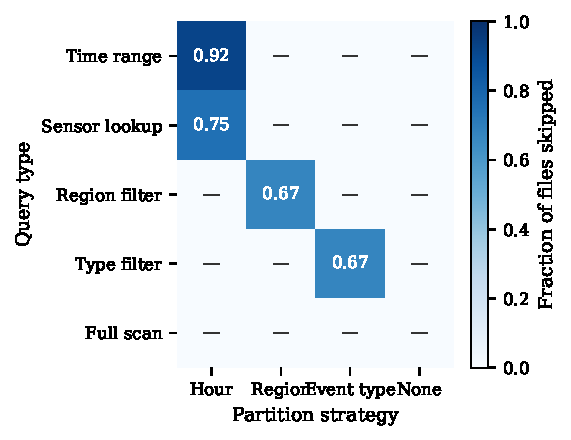
\includegraphics[width=0.50\linewidth]{charts/fig_pruning_matrix}
\caption{\label{fig:pruning}\textbf{Partition pruning matrix.}
  Fraction of Parquet files skipped at query time for each
  query-type--partition-strategy combination. Cell colour encodes the
  pruning ratio; dashes indicate zero pruning. Time-range queries
  achieve the highest pruning (92\%) under hourly partitioning;
  full-scan queries are irreducible under all strategies. Values are
  assumed rather than measured.}
\end{figure}

\FloatBarrier

\subsection*{Reward function}

The reward function comprises three independently computed signals.

\textbf{Compact reward} (Eq.~\ref{eq:compact}):
\begin{equation}
r_c = -w_f \tilde{f} + w_u u - w_c \tilde{a}_c + w_\tau \tau(a, r),
\label{eq:compact}
\end{equation}
where $\tilde{f} = \min(f / F_{\max}, 1)$, $u$ is block utilisation,
$\tilde{a}_c$ is the normalised compaction action cost, and
$\tau(a, r)$ is the target-size bonus depending on action $a$ and
ingestion rate $r$. Weights: $w_f = 0.25$, $w_u = 0.20$,
$w_c = 0.10$, $w_\tau = 0.45$.

\textbf{Partition reward} (Eq.~\ref{eq:partition}):
\begin{equation}
r_p = w_p p + w_{\Delta p} \Delta p - w_s \tilde{s}
    - w_{cp} \tilde{a}_p,
\label{eq:partition}
\end{equation}
where $p$ is the current partition pruning ratio,
$\Delta p = \bar{p}_t - \bar{p}_{t-1}$ is the pruning improvement,
$\tilde{s}$ is normalised partition skew, and $\tilde{a}_p$ is the
normalised partition action cost. Weights: $w_p = 0.55$,
$w_{\Delta p} = 0.25$, $w_s = 0.10$, $w_{cp} = 0.10$.

\textbf{Global reward} (Eq.~\ref{eq:global}):
\begin{equation}
r_g = -w_\ell \tilde{\ell} - w_f \tilde{f} + w_p p + w_u u,
\label{eq:global}
\end{equation}
where $\tilde{\ell} = \min(\ell / L_{\max}, 1)$ with
$L_{\max} = 15{,}000$\,ms. Weights: $w_\ell = 0.30$, $w_f = 0.20$,
$w_p = 0.30$, $w_u = 0.20$. The global reward is the primary
evaluation target; compact and partition rewards serve as dedicated
training signals for the respective specialists.

These weights were chosen to balance the four components on a common
scale rather than derived from a cost measurement. We therefore report a
sensitivity analysis in which each weight is perturbed by $\pm$25\% and
all four renormalised, with the global reward recomputed per step from
logged metrics and all policies re-ranked. We also note explicitly in
Limitations that training on $r_c$ and $r_p$ while evaluating on $r_g$
constitutes an objective mismatch, and identify the specific term
responsible.

\FloatBarrier

\subsection*{Hierarchical architecture}

The framework comprises three tiers: the \env{} environment, a
rule-based meta-controller, and two specialist RL agents coordinated
through a shared model registry (Fig.~\ref{fig:architecture}). The
arbitration tier is \emph{not} learned; the two specialists are.

\textbf{Meta-controller.}
The meta-controller computes two urgency scores at each step and
delegates:
\begin{equation}
\delta = \begin{cases}
\text{COMPACTION} & \text{if } u_c \geq u_p \geq \theta \\
\text{PARTITION}  & \text{if } u_p > u_c \geq \theta \\
\text{NOOP}       & \text{otherwise,}
\end{cases}
\end{equation}
where $\theta = 0.35$ is the minimum urgency threshold.

Compaction urgency $u_c$ is a piecewise-linear function of file count $f$:
\begin{equation}
u_c(f) = \begin{cases}
0.95 & f \geq 96 \\[2pt]
0.60 + 0.35 \cdot \dfrac{f - 36}{60} & 36 \leq f < 96 \\[6pt]
0.10 + 0.50 \cdot \dfrac{f - 12}{24} & 12 \leq f < 36 \\[2pt]
0    & f < 12,
\end{cases}
\end{equation}
with a $+$0.15 boost when block utilisation falls below 0.55.
A 4-step cooldown prevents repeated compaction.

Partition urgency $u_p$ accumulates from three signals: $+$0.40 if
$\bar{p} < 0.25$, $+$0.30 if the dominant query-type fraction exceeds
0.45, and $+$0.10 if the partition layout has not changed for more than
100 steps. A 20-step cooldown prevents partition thrashing. Urgency is
zeroed if $\bar{p} > 0.50$. Every constant named here is swept in
Table~\ref{tab:meta}.

\textbf{Neural architectures.}
All architectures accept input of shape $(\text{batch}, W, F)$ and
expose a common interface returning an action distribution and a scalar
state-value estimate.

\textit{\attentive{}} uses a Transformer-style
encoder\textsuperscript{10}:
input $\to$ Dense(64, ReLU) $+$ trainable positional encoding
$\to$ multi-head self-attention (4 heads, key dimension 64,
dropout 0.1) $+$ residual $+$ LayerNorm
$\to$ FFN (128$\to$64, ReLU, dropout 0.1) $+$ residual $+$ LayerNorm
$\to$ global average pooling $\to$ actor Dense($N_a$, softmax) and
critic Dense(1).

\textit{\mlpppo{}} is a feedforward actor-critic:
input $\to$ Flatten $\to$ Dense(256, ReLU) $\to$ Dense(128, ReLU)
$\to$ Dropout(0.1); actor: Dense(64, ReLU) $\to$ Dense($N_a$, softmax);
critic: Dense(64, ReLU) $\to$ Dense(1).
\textit{\matchedmlp{}}, used as the capacity control in
Section~\ref{sec:attention}, is the same topology with hidden widths
solved per specialist to match \attentive{}'s parameter count to within
0.06\% --- $(128, 288)$ for compaction and $(128, 192)$ for partition.

\textit{\ddqn{}} is a dueling double DQN\textsuperscript{11,29}:
input $\to$ Flatten $\to$ Dense(256, ReLU) $\to$ BatchNorm $\to$
Dense(128, ReLU) $\to$ BatchNorm; value stream: Dense(64, ReLU) $\to$
$V(s)$; advantage stream: Dense(64, ReLU) $\to$ $A(s,a)$. The streams
are aggregated using the standard mean-centred form
(Eq.~\ref{eq:dueling}):
\begin{equation}
Q(s,a) = V(s) + \left( A(s,a)
  - \frac{1}{|\mathcal{A}|}\sum_{a'} A(s,a') \right).
\label{eq:dueling}
\end{equation}
The Double-DQN target uses the online network to select the next action
and the target network to evaluate it (Eq.~\ref{eq:ddqn}):
\begin{equation}
y = r + \gamma\, Q_{\theta^-}\!\left(s',
  \arg\max_{a'} Q_{\theta}(s', a')\right)(1 - d),
\label{eq:ddqn}
\end{equation}
with the target network synchronised every 50 gradient steps.
For interface uniformity the model additionally exposes
$\mathrm{softmax}(Q)$; all value updates operate on raw $Q$-values
(this was the site of the online-adaptation defect reported in
Section~\ref{sec:adaptive}).

\begin{figure}[!htbp]
  \centering
  \begin{subfigure}[t]{0.47\textwidth}
    \centering
    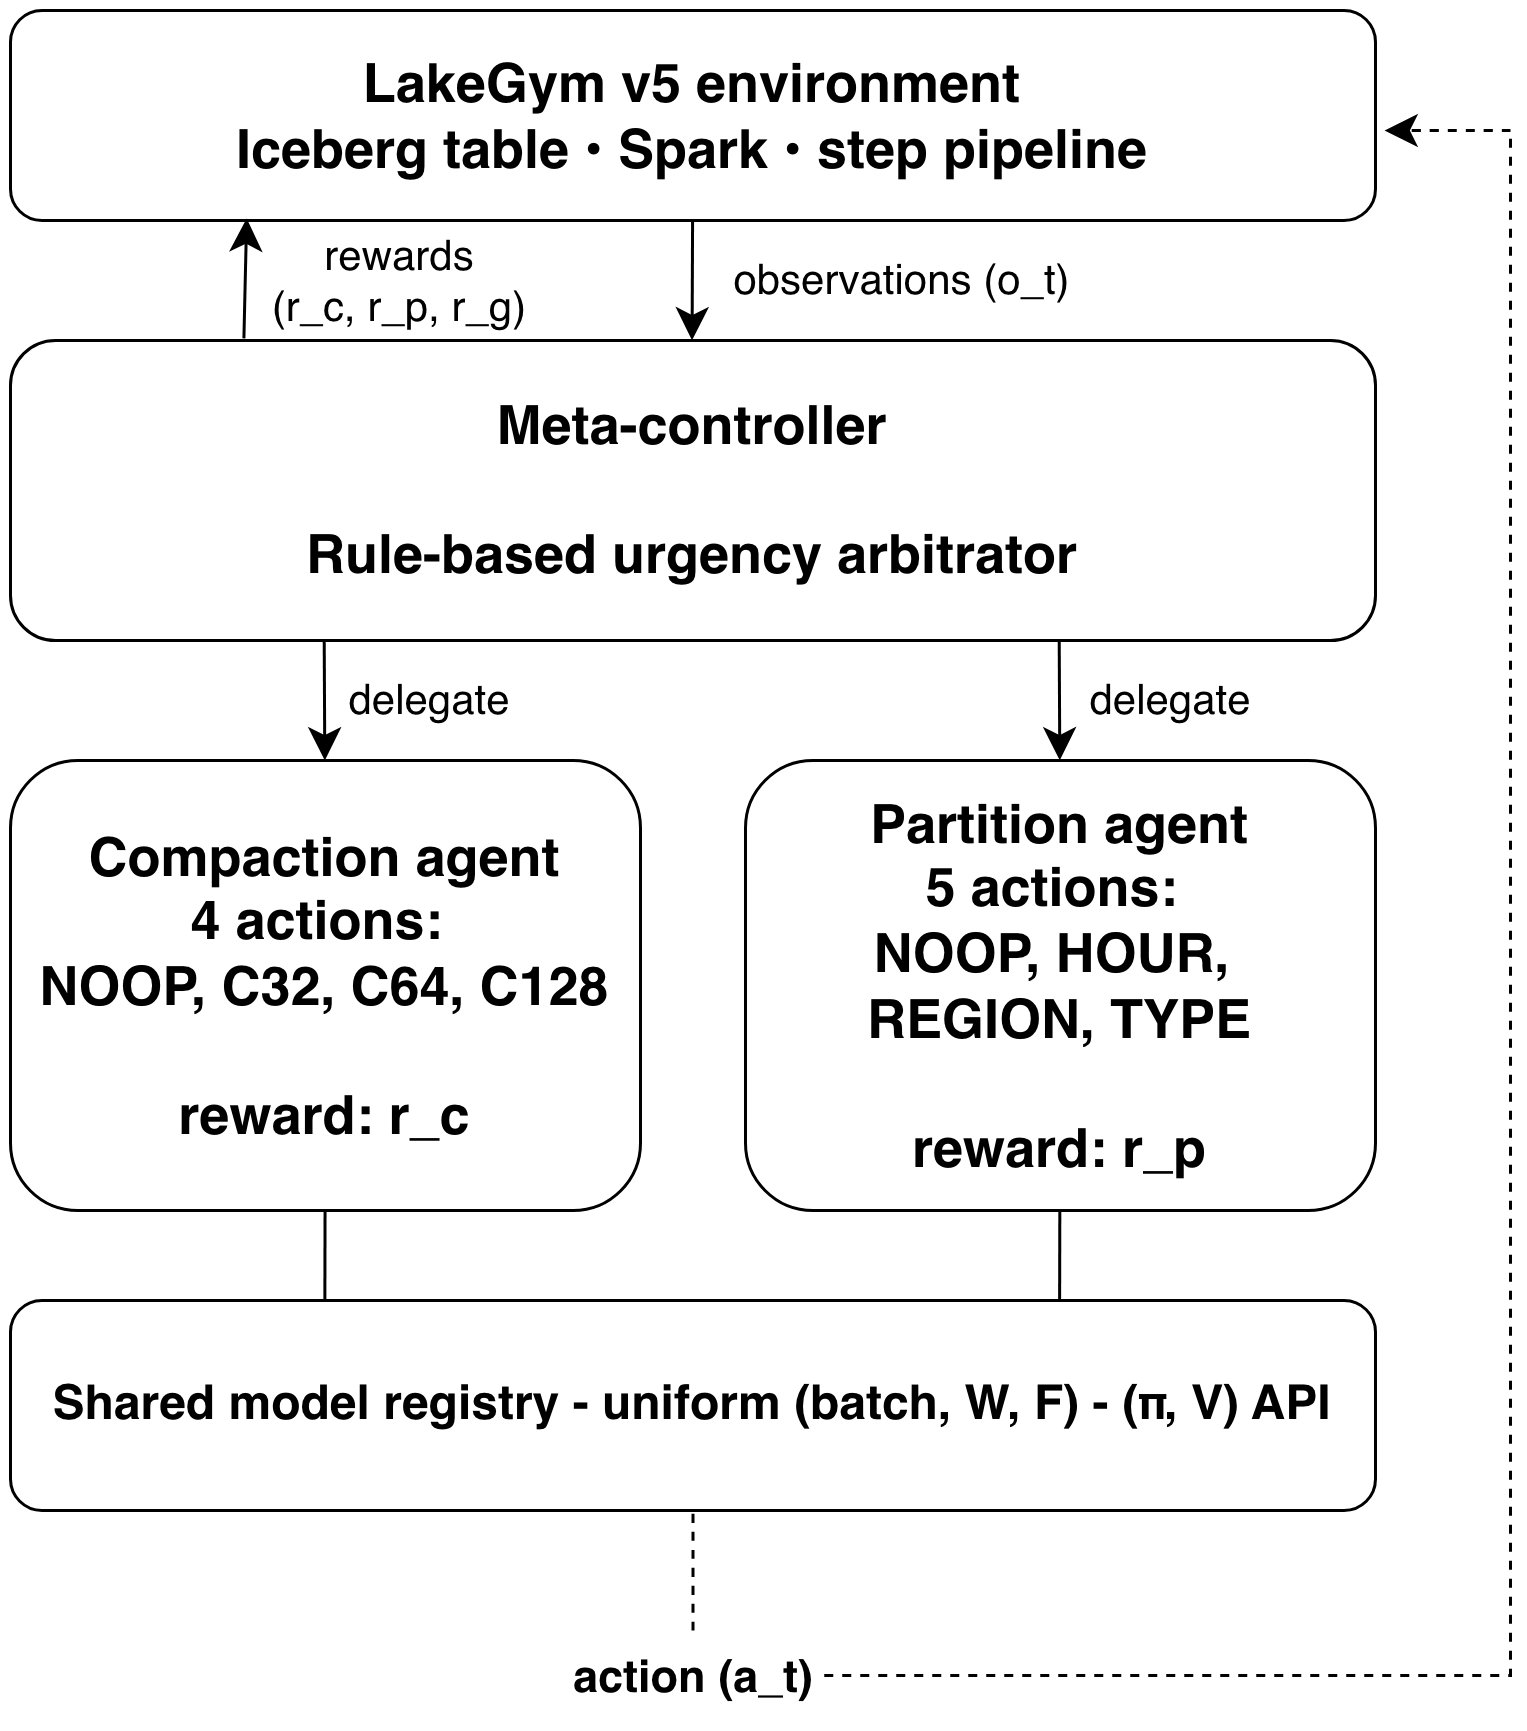
\includegraphics[width=\linewidth]{charts/fig_arch_system}
    \caption{\textbf{Hierarchical system flow.}
    The rule-based meta-controller computes urgency scores and delegates
    to one of two learned specialists, or takes no action.}
    \label{fig:architecture}
  \end{subfigure}
  \hfill
  \begin{subfigure}[t]{0.47\textwidth}
    \centering
    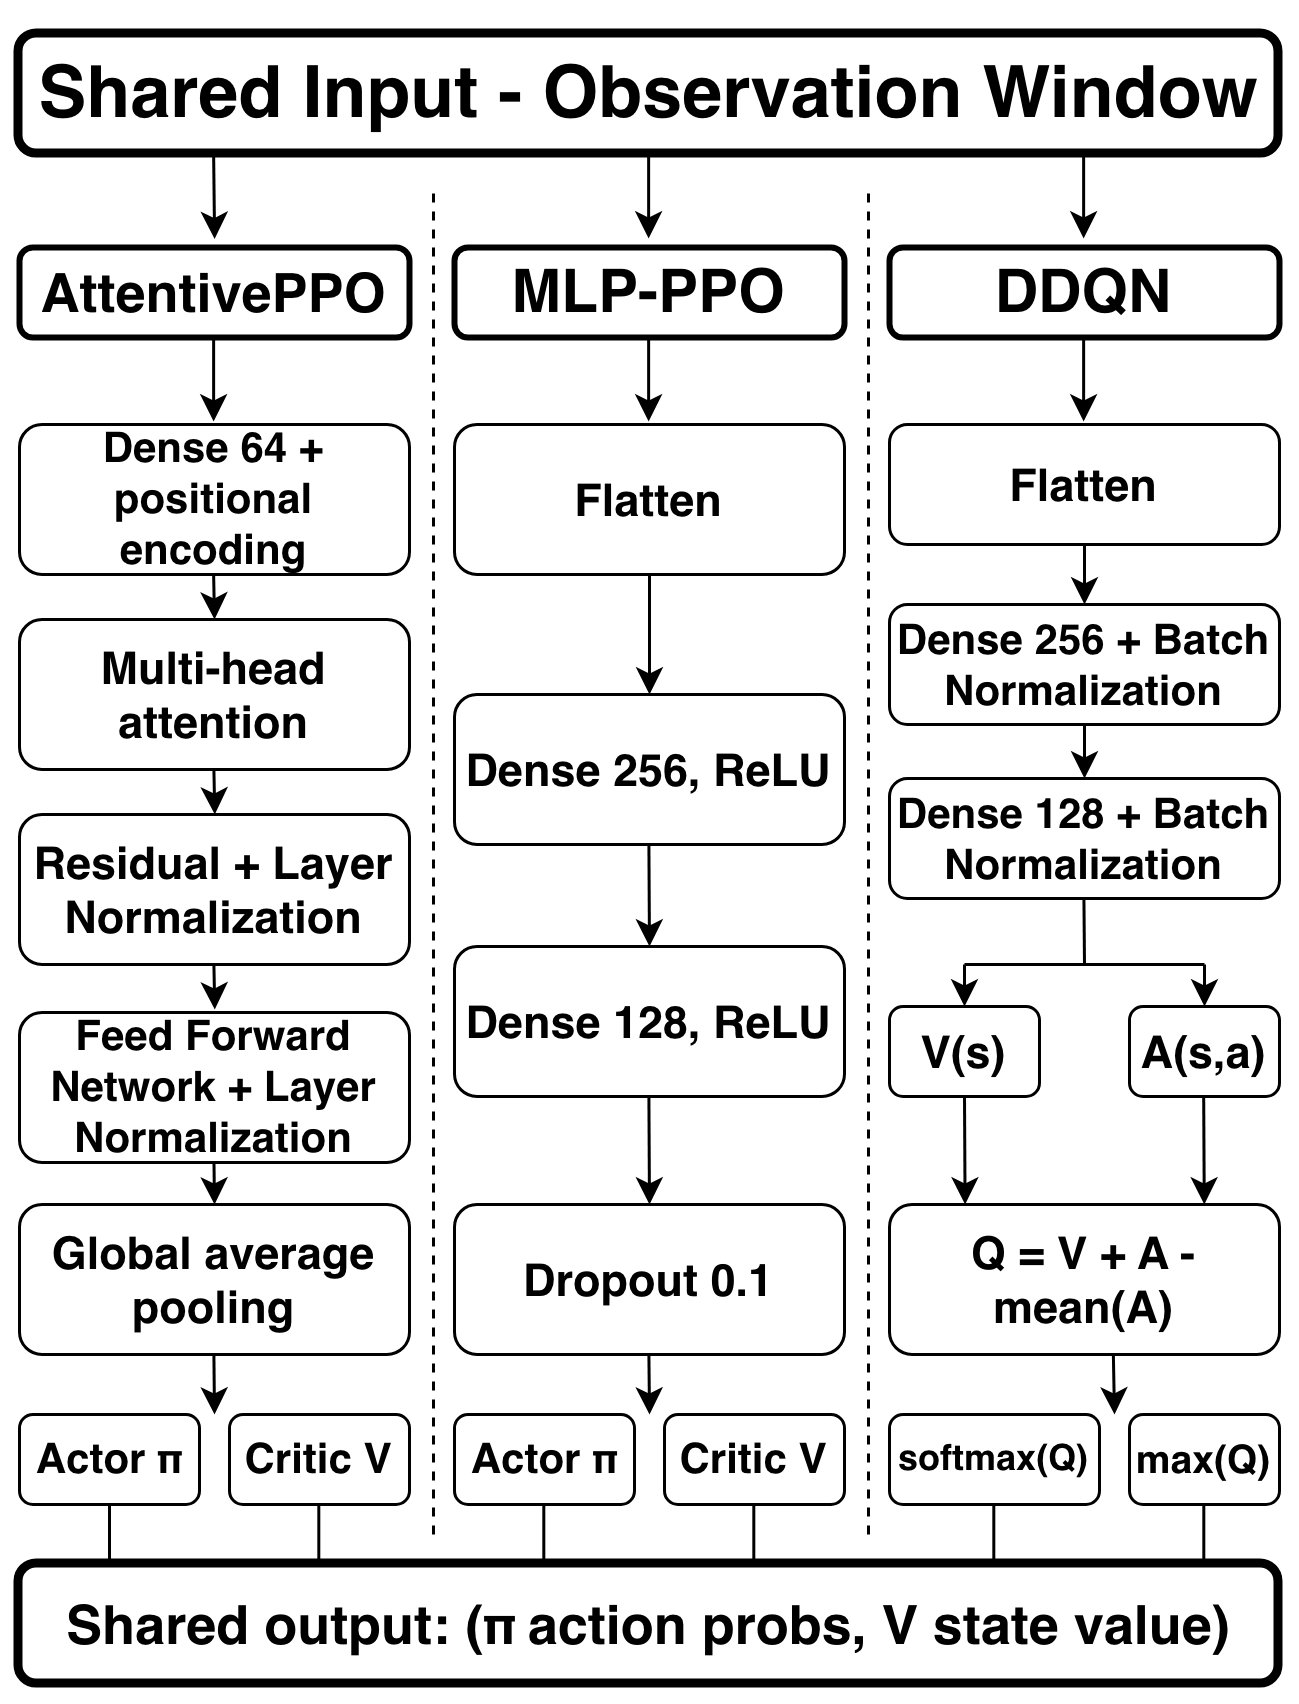
\includegraphics[width=\linewidth]{charts/fig_arch_models}
    \caption{\textbf{Neural candidate comparison.}
    The three structural paradigms---attention, feedforward, and
    dueling---sharing a common input--output interface.}
    \label{fig:arch_models}
  \end{subfigure}
  \caption{System architecture and neural model comparison.}
  \label{fig:both}
\end{figure}

\FloatBarrier

\subsection*{Training procedure}

Specialists are trained offline on logged trajectories. The compaction
specialist ($W = 10$, $F = 8$, 4 actions) is trained on 14 baseline
episodes comprising 17{,}000 transitions; the partition specialist
($W = 20$, $F = 14$, 5 actions) is trained on 6 partition-active
episodes comprising 4{,}990 transitions. Both pools are augmented with
counterfactual recovery trajectories added during this revision to break
the trajectory-identity shortcut described in Results.

Three corrections to the original procedure are applied uniformly across
all architectures. Staleness features are capped so they cannot encode
unbounded trajectory provenance. Normalisation constants are shared
between training and serving. Actions are sampled in a balanced manner
during offline training, and advantages are standardised per action, so
that the majority \noop{} class cannot dominate the objective.

To make the architecture comparison in Table~\ref{tab:threeway}
meaningful, all three architectures use an identical configuration:
the same data pools, 150 epochs for the compaction specialist and 200
for the partition specialist, batch size 64, and the same five random
seeds $\{1,2,3,4,5\}$. Architecture-specific hyperparameters are listed
in Table~\ref{tab:hyper}. Because the objectives differ by architecture
(offline PPO-clip for the two actor-critics, Double-DQN for the
value-based model), the comparison is between architecture--objective
pairings and not between encoders in isolation; the capacity-matched
control in Table~\ref{tab:matched} isolates the encoder specifically.

\begin{table}[!htbp]
\centering
\setlength{\tabcolsep}{4pt}
\begin{tabular}{llccccc}
\toprule
\textbf{Variant} & \textbf{Objective} & \textbf{LR} & $\gamma$ &
  \textbf{Entropy} & \textbf{Clip / target} & \textbf{Params} \\
\midrule
\attentive{} (compaction) & offline PPO-clip & $3\times10^{-4}$ & 0.95 & 0.01 & --- & 84{,}741 \\
\attentive{} (partition)  & offline PPO-clip & $3\times10^{-4}$ & 0.99 & 0.10 & --- & 85{,}830 \\
\mlpppo{} (compaction)    & offline PPO-clip & $3\times10^{-4}$ & 0.95 & 0.01 & clip 0.2 & 70{,}469 \\
\mlpppo{} (partition)     & offline PPO-clip & $3\times10^{-4}$ & 0.99 & 0.10 & clip 0.2 & 121{,}734 \\
\ddqn{} (compaction)      & Double DQN & $1\times10^{-4}$ & 0.95 & --- & target 50 & 71{,}237 \\
\ddqn{} (partition)       & Double DQN & $1\times10^{-4}$ & 0.99 & --- & target 50 & 122{,}502 \\
\bottomrule
\end{tabular}
\caption{\label{tab:hyper}\textbf{Hyperparameters.}
  All variants share: 150 epochs (compaction) / 200 epochs
  (partition), batch size 64, per-action advantage standardisation,
  balanced action sampling, and seeds $\{1,2,3,4,5\}$. Window sizes are
  $W=10$ (compaction) and $W=20$ (partition); feature counts are $F=8$
  and $F=14$. The complete appendix is included in the archived
  repository.}
\end{table}

\textbf{Online adaptation.}
For the experiments in Section~\ref{sec:adaptive}, agents begin from a
frozen checkpoint and update weights during rollout: PPO for the two
actor-critics and Double-DQN with a replay buffer for \ddqn{}. The
exploration rate decays from $\varepsilon = 0.10$ over 200 environment
steps, decremented once per environment step.

\FloatBarrier

\subsection*{Baseline policies}

We evaluate 14 heuristic compaction policies, 3 workload-aware
heuristics, and 2 ablation policies (Table~\ref{tab:baselines}).
Heuristics include always-compact variants (C32, C64, C128), periodic
compaction (every 5 or 10 steps), threshold-triggered compaction (file
count $>10$ or $>20$), random compaction, and adaptive compaction with
frequency proportional to file growth rate. Ablation policies use the
\attentive{} architecture restricted to the relevant action sub-space.

\begin{table}[!htbp]
\centering
\renewcommand{\arraystretch}{0.85}
\begin{tabular}{lp{8cm}}
\toprule
\textbf{Policy} & \textbf{Description} \\
\midrule
\texttt{No\_Maintenance}          & Takes no action at any step \\
\texttt{AlwaysCompact}            & Compacts every step with \texttt{64KB} \\
\texttt{AlwaysCompact\_C32}       & Compacts every step with \texttt{32KB} \\
\texttt{AlwaysCompact\_C128}      & Compacts every step with \texttt{128KB} \\
\texttt{Periodic5\_C64}           & Compacts every 5 steps with \texttt{64KB} \\
\texttt{Periodic10\_C64}          & Compacts every 10 steps with \texttt{64KB} \\
\texttt{Periodic10\_C32}          & Compacts every 10 steps with \texttt{32KB} \\
\texttt{Periodic10\_C128}         & Compacts every 10 steps with \texttt{128KB} \\
\texttt{Threshold10\_C32}         & Compaction for file count $> 10$ (\texttt{32KB}) \\
\texttt{Threshold10\_C64}         & Compaction for file count $> 10$ (\texttt{64KB}) \\
\texttt{Threshold10\_C128}        & Compaction for file count $> 10$ (\texttt{128KB}) \\
\texttt{Threshold20\_C64}         & Compaction for file count $> 20$ (\texttt{64KB}) \\
\texttt{Random\_Compact}          & Uniformly samples a compaction action \\
\texttt{AdaptiveCompaction}       & Proportional frequency based on file growth \\
\midrule
\texttt{WorkloadAwareThreshold}   & Dual-aware thresholding and partitioning \\
\texttt{PartitionExploration}     & Sequential cycle of partitioning strategies \\
\texttt{Random\_Partition}        & Uniformly samples a partition action \\
\bottomrule
\end{tabular}
\caption{\label{tab:baselines}\textbf{Heuristic baseline strategies.}
  Fourteen rule-based compaction methods and three workload-aware
  benchmarks used for comparison. \texttt{WorkloadAwareThreshold} is the
  strongest baseline and is used as the reference in all headline
  comparisons.}
\end{table}

\FloatBarrier

\subsection*{Evaluation protocol and statistical analysis}

\textbf{Seeding and pairing.}
Each RL architecture is trained with five independent random seeds. Each
resulting agent is evaluated on five episodes, giving 25 episodes per
policy. Environment seeds are a deterministic function of (protocol,
seed slot, episode index) and are \emph{independent of the policy}, so
every policy is evaluated on an identical set of episodes and all
comparisons are paired. Heuristic policies are evaluated on the same
environment seeds.

\textbf{Protocols.}
The primary protocol is the 500-step evaluation workload; the 1{,}000-step
standard workload is reported as a concordance check (Spearman
$\rho = 0.964$). Held-out protocols \texttt{drift500} and
\texttt{mixed500} are described above.

\textbf{Statistical methods.}
Uncertainty on means is reported as percentile bootstrap 95\% confidence
intervals with 10{,}000 resamples\textsuperscript{32} computed over
independent episodes, never over autocorrelated within-episode steps.
Across-seed standard deviation is reported separately, because it
measures training-run variability that a confidence interval on the
pooled mean does not. Paired comparisons use both the Wilcoxon
signed-rank test and an exact paired permutation test; effect sizes are
Cliff's $\delta$\textsuperscript{34} with thresholds 0.147 (small), 0.33
(medium) and 0.474 (large). Multiplicity is controlled with
Holm--Bonferroni correction\textsuperscript{33} within each comparison
family. Where a design cannot reach $p < 0.05$ --- the sensitivity sweep
($n=3$, floor $p = 0.25$) and the generalization study ($n=5$, floor
$p = 0.0625$) --- we report intervals and effect sizes and state that the
study is powered for estimation rather than hypothesis testing.

\textbf{Data integrity.}
A Spark driver crash does not raise inside the simulator: metric
collection returns zero and the query returns a latency of $-1$, which
the reward formula maps to exactly 0.0, so a dead run can be written out
with a successful status. We therefore audit every run before analysis
with a validator that rejects any episode with non-positive mean
latency, zero mean file count, absurd latency ($>60{,}000$\,ms), or
identical latency across all episodes of a seed. All 216 evaluation runs
reported here pass; runs that failed were deleted and re-executed under
per-seed process isolation. The validator is included in the archived
repository.

\textbf{Cost model.}
$C = C_q \sum_t \ell_t + C_c N_c + C_s \sum_t \sigma_t$, where
$C_q = \$0.00001$/ms, $C_c = \$0.005$ per compaction operation,
$C_s = \$0.000001$/KB-step, $\ell_t$ is per-step latency, $N_c$ is total
compaction operations, and $\sigma_t$ is table size in KB at step $t$.
Table~\ref{tab:cost} adds inference at \$0.096/h CPU and offline
training at \$0.526/h GPU amortised over 100 deployment episodes. We
note that a flat per-operation compaction charge under-charges
aggressive strategies relative to production, where a compaction is a
distributed rewrite whose cost grows with bytes touched; we therefore
also evaluate a size-proportional variant calibrated to the same mean,
which leaves the ordering essentially unchanged at this simulation's
scale.

\FloatBarrier

% ════════════════════════════════════════════════════════════════════════════
\section*{References}
% ════════════════════════════════════════════════════════════════════════════

\begin{enumerate}

\item Blue, R., Weeks, D., Reid, J. \& Steinbach, C. Iceberg: A fast and
  expressive table format for large, slow tables. In \textit{Proc. ACM
  SIGMOD} 3434--3441 (ACM, 2020).

\item Armbrust, M. \textit{et al.} Delta Lake: High-performance ACID table
  storage over cloud object stores. \textit{Proc. VLDB Endow.}
  \textbf{13}, 3411--3424 (2020).

\item Chandar, V., Rao, B. S. \& Agarwal, N. Apache Hudi: The data lake
  platform. \textit{arXiv} preprint arXiv:2301.09517 (2023).

\item Kraska, T. \textit{et al.} The case for learned index structures. In
  \textit{Proc. ACM SIGMOD} 489--504 (ACM, 2018).

\item Agrawal, S. \textit{et al.} Database tuning advisor for Microsoft SQL
  Server 2005. In \textit{Proc. VLDB} 1110--1121 (2004).

\item Marcus, R. \& Papaemmanouil, O. Re-Join: How the machine learned to
  join. In \textit{Workshop on ML for Progressively Learned Databases
  (NIPS DBLearn)} (2018).

\item Trummer, I. \textit{et al.} SkinnerDB: Regret-bounded query evaluation
  via reinforcement learning. In \textit{Proc. ACM SIGMOD} 1153--1170
  (ACM, 2019).

\item Van Aken, D., Pavlo, A., Gordon, G. J. \& Zhang, B. Automatic
  database management system tuning through large-scale machine learning.
  In \textit{Proc. ACM SIGMOD} 1009--1024 (ACM, 2017).

\item Zhang, J. \textit{et al.} An end-to-end automatic cloud database
  tuning system using deep reinforcement learning. In \textit{Proc. ACM
  SIGMOD} 415--432 (ACM, 2019).

\item Vaswani, A. \textit{et al.} Attention is all you need. In
  \textit{Advances in Neural Information Processing Systems (NeurIPS)}
  vol.~30 (2017).

\item Wang, Z. \textit{et al.} Dueling network architectures for deep
  reinforcement learning. In \textit{Proc. ICML} 1995--2003 (2016).

\item Dayan, N., Athanassoulis, M. \& Idreos, S. Dostoevsky: Better
  space-time trade-offs for LSM-tree based key-value stores via adaptive
  removal of superfluous merging. In \textit{Proc. ACM SIGMOD} 505--520
  (ACM, 2018).

\item Schulman, J. \textit{et al.} Proximal policy optimization algorithms.
  \textit{arXiv} preprint arXiv:1707.06347 (2017).

\item Camacho-Rodr\'{\i}guez, J. \textit{et al.} LST-Bench: Benchmarking
  Log-Structured Tables in the Cloud. In \textit{Proc. ACM SIGMOD}
  1--14 (ACM, 2024).

\item Armbrust, M. \textit{et al.} Lakehouse: A New Generation of Open
  Platforms that Unify Data Warehousing and Advanced Analytics. In
  \textit{Proc. CIDR} (2021).

\item Yang, Z. \textit{et al.} Qd-tree: Learning Data Layouts for Big
  Data Analytics. In \textit{Proc. ACM SIGMOD} 170--184 (ACM, 2020).

\item Kraska, T. \textit{et al.} SageDB: A Learned Database System. In
  \textit{Proc. CIDR} (2019).

\item Pavlo, A. \textit{et al.} Self-Driving Database Management Systems.
  In \textit{Proc. CIDR} (2017).

\item Marcus, R. \textit{et al.} Neo: A Learned Query Optimizer.
  \textit{Proc. VLDB Endow.} \textbf{12}, 1705--1718 (2019).

\item Li, G. \textit{et al.} QTune: A Query-Aware Database Tuning System
  with Deep Reinforcement Learning. \textit{Proc. VLDB Endow.}
  \textbf{12}, 2118--2130 (2019).

\item Kanellis, K. \textit{et al.} LlamaTune: Sample-Efficient DBMS
  Configuration Tuning. \textit{Proc. VLDB Endow.} \textbf{15},
  2726--2738 (2022).

\item Cai, B. \textit{et al.} HUNTER: An Online Cloud Database Hybrid
  Tuning System for Personalized Requirements. In \textit{Proc. ACM
  SIGMOD} 625--638 (ACM, 2022).

\item Yang, Z. \textit{et al.} HWTune: A Hardware-Aware Database Tuning
  System with Deep Reinforcement Learning. \textit{IEEE Trans. Knowl.
  Data Eng.} \textbf{36}, 2284--2297 (2023).

\item Feng, Y. \textit{et al.} CTuner: Automatic NoSQL Database Tuning
  with Causal Reinforcement Learning. In \textit{Proc. ACM SIGKDD}
  1--12 (ACM, 2024).

\item Liu, Y. \textit{et al.} MLETune: Streamlining Database Knob Tuning
  via Multi-LLMs Experts Guided Deep Reinforcement Learning.
  \textit{IEEE Access} \textbf{12}, 1--15 (2024).

\item Zhang, K., Yang, Z. \& Ba\c{s}ar, T. Multi-Agent Reinforcement
  Learning: A Selective Overview of Theories and Algorithms.
  \textit{J. Mach. Learn. Res.} \textbf{22}, 1--85 (2021).

\item Vezhnevets, A. S. \textit{et al.} FeUdal Networks for Hierarchical
  Reinforcement Learning. In \textit{Proc. ICML} 3540--3549 (2017).

\item Wang, Y. \textit{et al.} A highly efficient distributed database
  knobs tuning method based on multi-agent deep reinforcement learning.
  \textit{J. Supercomput.} (2025).

\item van Hasselt, H., Guez, A. \& Silver, D. Deep reinforcement learning
  with double Q-learning. In \textit{Proc. AAAI} 2094--2100 (2016).

\item Bacon, P.-L., Harb, J. \& Precup, D. The option-critic
  architecture. In \textit{Proc. AAAI} 1726--1734 (2017).

\item Peng, X. B., Kumar, A., Zhang, G. \& Levine, S.
  Advantage-weighted regression: simple and scalable off-policy
  reinforcement learning. \textit{arXiv} preprint arXiv:1910.00177
  (2019).

\item Efron, B. \& Tibshirani, R. J. \textit{An Introduction to the
  Bootstrap} (Chapman \& Hall, 1993).

\item Holm, S. A simple sequentially rejective multiple test procedure.
  \textit{Scand. J. Stat.} \textbf{6}, 65--70 (1979).

\item Cliff, N. Dominance statistics: Ordinal analyses to answer ordinal
  questions. \textit{Psychol. Bull.} \textbf{114}, 494--509 (1993).

\end{enumerate}

% ════════════════════════════════════════════════════════════════════════════
\section*{Data availability}
% ════════════════════════════════════════════════════════════════════════════
The datasets generated and analysed during the current study, including
all experimental metrics collected across workload profiles, every
per-run manifest, and the model weights for all seeds, are archived at
Zenodo under DOI
\href{https://doi.org/10.5281/zenodo.21860273}{10.5281/zenodo.21860273}
and are additionally available in the LakePilot repository at
\url{https://github.com/OmarEssameldinMousa/LakePilot-Research-prototype}.
No pre-existing external datasets were used in this study; all data was
synthetically generated by the \env{} environment as described in the
Methods section.

% ════════════════════════════════════════════════════════════════════════════
\section*{Code availability}
% ════════════════════════════════════════════════════════════════════════════
The \env{} simulation environment, the meta-controller implementation,
the model registry, all training and evaluation scripts, the statistical
analysis pipeline, and the data-integrity validator are archived at
Zenodo under DOI
\href{https://doi.org/10.5281/zenodo.21860273}{10.5281/zenodo.21860273}
(release \texttt{v1.0-revision}) and are available under the MIT licence
at
\url{https://github.com/OmarEssameldinMousa/LakePilot-Research-prototype}.
The deposit pins the exact software environment used for every reported
result (Python 3.10.12, Apache Spark 3.5.7, PySpark 3.5.7,
TensorFlow 2.20.0, NumPy 2.2.6, pandas 2.3.3) and includes end-to-end
reproduction instructions. Every run carries a \texttt{manifest.json}
recording its random seed, configuration, git commit, hardware and
wall-clock time.

% ════════════════════════════════════════════════════════════════════════════
\section*{Acknowledgements}
% ════════════════════════════════════════════════════════════════════════════

The authors developed the \env{} simulation environment utilising the
open-source Apache Iceberg and Apache Spark frameworks.
All figures were generated using Matplotlib
(v3.8, \url{https://matplotlib.org}).

\section*{Funding}
This research did not receive any specific grant from funding agencies
in the public, commercial, or not-for-profit sectors.

% ════════════════════════════════════════════════════════════════════════════
\section*{Author contributions statement}
% ════════════════════════════════════════════════════════════════════════════

O.E.\ conceived the idea, implemented the \env{} environment,
developed the lakehouse solution, and designed the whole experiments.
O.K.\ implemented and trained the AI models.
O.S.\ assisted in baseline analysis and overall project execution.
A.Z.B.\ supervised the research.
All authors reviewed and approved the final manuscript.

% ════════════════════════════════════════════════════════════════════════════
\section*{Additional information}
% ════════════════════════════════════════════════════════════════════════════

\textbf{Competing interests.} The authors declare no competing interests.

\end{document}
